\documentclass{article}
\usepackage[utf8]{inputenc}
\usepackage{graphicx}
\usepackage{amsmath}
\renewcommand{\contentsname}{Indice dei contenuti}
\newcommand{\subsubsubsection}[1]{\paragraph{#1}\mbox{}\\}
\setcounter{secnumdepth}{4}
\setcounter{tocdepth}{4}
\title{Appunti (G) di Reti di Calcolatori}
\author{proff. D. Malandrino, R. Zaccagnino}
\date{a.a. 2020/2021}

\begin{document}

\maketitle

\tableofcontents

\section{Overview}
    L’espressione \textit{comunicazione dati} fa riferimento allo scambio (locale o remoto) di informazione fra due dispositivi attraverso un canale di comunicazione, il quale è caratterizzato da un mezzo trasmissivo (come un cavo). Affinché la comunicazione abbia luogo è necessario che i dispositivi siano parte di un sistema di comunicazione fatto di hardware e di software.

    \vspace{3mm}
    
    Un sistema di comunicazione è composto da \textit{messaggio} (i dati che devono essere inviati), \textit{mittente} (dispositivo che spedisce il messaggio), \textit{destinatario} (dispositivo che riceve il messaggio), \textit{mezzo trasmissivo} (cammino fisico sul quale il messaggio viaggia) e \textit{protocollo} (insieme di regole, adottate dai dispositivi) che governano la comunicazione).
    
    \vspace{3mm}
    
    Il \textbf{messaggio}, e cioè l'\textbf{informazione}, può essere rappresentata in varie forme, quali testi, numeri, immagini, audio, video e altro. Un messaggio è in \textit{forma discreta} se è rappresentato da sequenze di bit. Ad esempio, per il testo, la forma discreta coincide con una codifica ASCII; per le immagini, la forma discreta coincide con l'aggregazione di pixel.
    
    \vspace{3mm}
    
    La comunicazione fra due dispositivi può essere di tre tipi: \textbf{unidirezionale} (\textit{simplex}), \textbf{bidirezionale alternata} (\textit{duplex}) e \textbf{bidirezionale} (\textit{full-duplex}).
    
    \begin{itemize}
        \item 
        \textbf{Simplex:} La comunicazione avviene in una sola direzione, come succede al traffico automobilistico in una strada a senso unico. Solo uno dei due dispositivi può spedire dati mentre l’altro dispositivo può solo riceverli.
    
        \item
        \textbf{Duplex:} Ogni dispositivo può sia trasmettere che ricevere ma non contemporaneamente.
        
        \item
        \textbf{Full-Duplex:} Entrambi i dispositivi possono spedire e ricevere i dati contemporaneamente.
    \end{itemize}
    
    \subsection{Definizione di rete e connessione}
    
        Una \textbf{rete di calcolatori} (concettualmente nata col telegrafo nel 1840) è un insieme di dispositivi (detti \textit{nodi}) indipendenti ed interconnessi tra loro attraverso un canale di comunicazione, tramite il quale possono scambiarsi informazioni e cooperare. I vantaggi giacciono chiaramente nella possibilità di condividere risorse e collaborare, riducendo dunque i costi e distribuendo in modo omogeneo il peso computazionale. 
        
        Inoltre, una rete può garantire affidabilità e \textit{fault tolerance} (significa che, nell'eventualità del crash di un nodo, si ha a disposizione una copia replicata del servizio affinché l'utente comunque accedere al medesimo servizio). Lo svantaggio è che tutto ciò richiede una gestione difficoltosa e complessa.
        
        \vspace{3mm}
        
        Le connessioni che collegano i nodi di una rete possono essere classificate in due
        grandi categorie: \textit{connessioni punto-punto} e \textit{connessioni multipunto}.
        
        \begin{itemize}
            \item 
            Una \textbf{connessione punto-punto} si ottiene dedicando un canale fisico ai due dispositivi che devono comunicare. L’intera capacità del canale è dedicata ai due dispositivi connessi dal
            collegamento. Un esempio pratico è un cavo che connette due computer.
            
            \item
            Una \textbf{connessione multipunto} è un collegamento condiviso da più di due dispositivi. La capacità di un collegamento multipunto va condivisa fra i dispositivi che lo usano. La condivisione può avvenire temporalmente se l’accesso al mezzo trasmissivo è esclusivo, motivo per cui l'utilizzo del collegamento è \textit{a turnazione}. 
            
            Se il canale trasmissivo ammette un utilizzo simultaneo da parte di più dispositivi allora si parla di \textit{condivisione dello spazio}.
        \end{itemize}
        
        La \textbf{topologia} descrive come i nodi sono fisicamente connessi da un mezzo trasmissivo, e possono essere di quattro tipi: \textit{mesh}, \textit{stella}, \textit{bus} e \textit{anello}. E' anche possibile elaborare soluzioni ibride.
        
        \begin{itemize}
            \item 
            In una topologia \textbf{mesh} (\textit{a maglia di rete}), ogni nodo ha un collegamento punto-punto con ogni altro nodo della rete. 
            
            Utilizzando dei collegamenti simplex occorrono \(n*(n-1)\) collegamenti per una mesh; invece, utilizzando dei collegamenti duplex occorrerebbero \(n*(n-1)/2\) collegamenti.
            
            Il numero di collegamenti è quadratico rispetto al numero di nodi.
            
            Il vantaggio è che ogni coppia di nodi può comunicare indipendentemente da ogni altra coppia, assicurando affidabilità e sicurezza. Lo svantaggio è che serviranno molti cavi per collegare i nodi.
            
            \begin{center}
                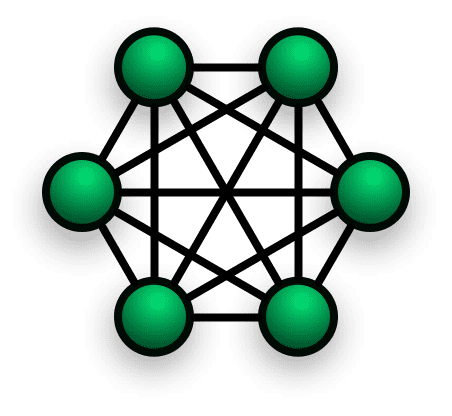
\includegraphics[scale=0.25]{images/MeshNetwork.png}
            \end{center}
            
            \item
            In una topologia a \textbf{stella}, ogni nodo è connesso con un collegamento punto-punto ad un dispositivo centrale chiamato \textbf{hub}. Tutto il traffico passa attraverso l'hub.
            
            E' una soluzione economica: se un nodo si rompe, non si compromette l'intera rete. Tuttavia, tutta la rete dipesa dall'hub, e se esso si rompe, l'intera rete diventa inutilizzabile.
            
            \begin{center}
                
\includegraphics[scale=0.090]{images/StarNetwork.png}
            \end{center}
            
            \item
            In una topologia a \textbf{bus}, la rete utilizza un collegamento multipunto per connettere tutti i nodi. Ogni nodo è connesso al bus tramite un connettore fisico. Quando il segnale attraversa il bus, il connettore riesce a leggerlo.
            
            Il connettore è detto \textit{dorsale}.
            
            Un esempio di topologia con bus è l'Ethernet.
            
            Se il connettore è troppo lungo, il segnale perde d'intensità, limitando notevolmente il numero di connettori e quindi di nodi che si possono collegare al bus. Il vantaggio di questa soluzione è la facilità di installazione di un nuovo nodo. In ogni caso, la gestione dei problemi relativi al bus in sé è difficoltosa e un guasto al connettore potrebbe blocare tutte le connessioni.
            
            Inoltre, l'amministratore di rete deve posizionare adeguatamente i nodi affinché i connettori siano distanziati e non entrino in conflitto.
            
            \begin{center}
                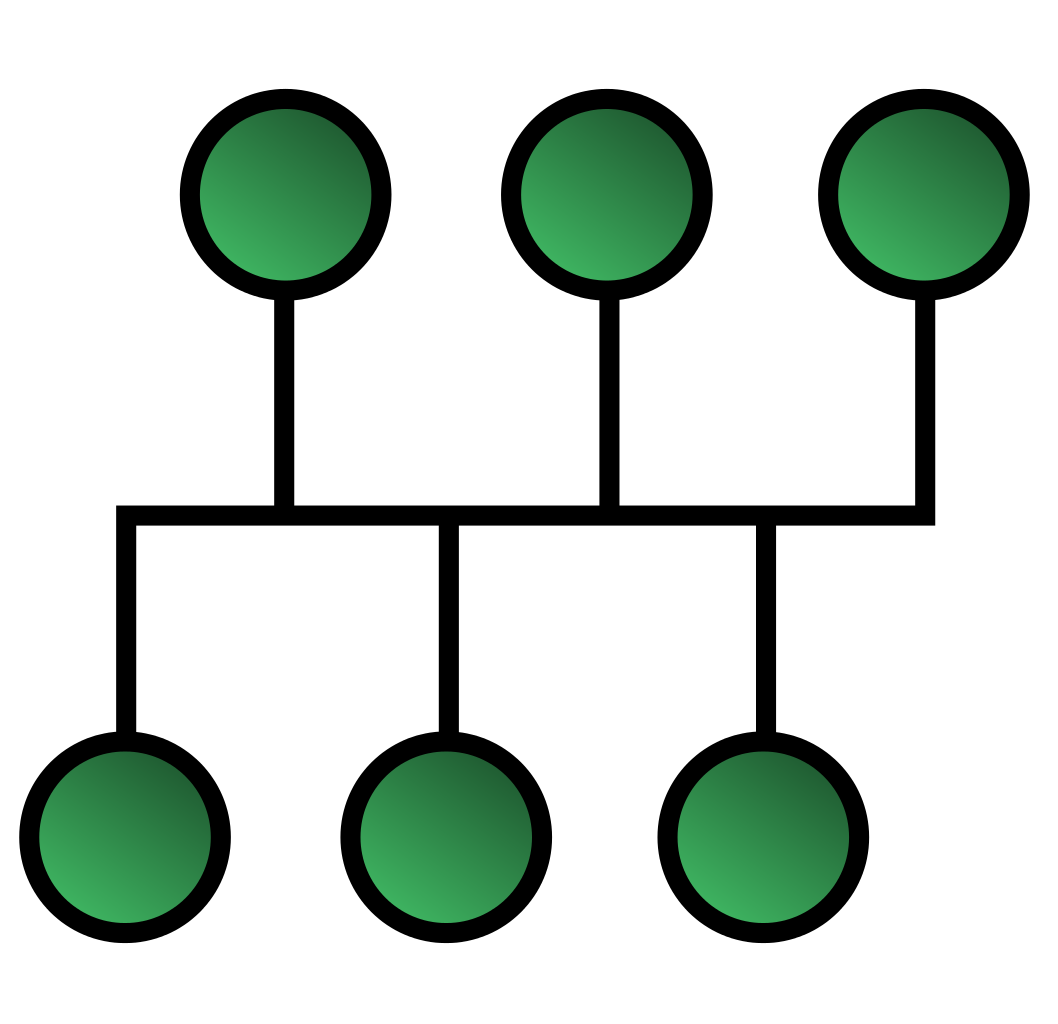
\includegraphics[scale=0.090]{images/BusNetwork.png}
            \end{center}
            
            \item
            In una topologia ad \textbf{anello}, ogni nodo ha un collegameno punto-punto con solo altri due nodi, cioè il nodo precedente e quello successivo. I dati viaggiano in una sola direzione, e ogni nodo ha un ripetitore che rigenera il segnale.
            
            Il vantaggio è che aggiungere un nodo o rimuoverlo richiede il cambiamento dei suoi due vicini e nient'altro; inoltre, isolare un guasto è molto semplice.
            
            Lo svantaggio è relativo alla natura unidirezionale del traffico. Se un ripetitore si rompe, l'intera rete diventa inutilizzabile. La soluzione al problema è l'aggiunta di un ulteriore anello, in modo tale da avere una comunicazione bidirezionale.
            
            \begin{center}
                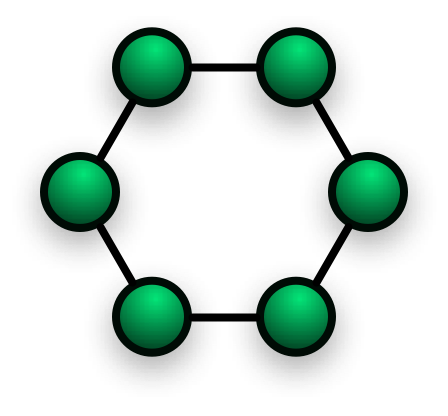
\includegraphics[scale=0.25]{images/RingNetwork.png}
            \end{center}
        \end{itemize}
        
        Le topologie ibride impiegano più tipi di topologie combinate.
    
    \subsection{Internet e Internet Service Providers}
    
        Una rete è categorizzabile anche in base alla sua dimensione (LAN, MAN, WAN, Interrete). Esistono molte "\textit{internet}", ma la più grande è "\textit{Internet}".
    
        \textbf{Internet} è una rete di reti che usa il protocollo TCP/IP (progenie del Dr. Vinton Cerf, citato per la prima volta nel 1974) e il \textit{Packet Switching} (i dati vengono impacchettati, suddivisi e seguono più percorsi per raggiungere la destinazione). 
        
        \vspace{3mm}
        
        La sua origine può essere datata al 1945 (grazie, fra gli altri, al pioniere Vannervar Bush, autore degli ipertesti - termine coniato in origine da Ted Nelson) e attribuita al progetto \textbf{Memex}, che si prefiggeva l'obiettivo di "\textit{mettere in relazione informazioni in maniera simile al cervello umano}", poi meglio concretizzato nella rete \textbf{ARPANET} degli Stati Uniti, il cui primo nodo è datato 1969 e che inizialmente connetteva fra i 4 e i 23 computer.
        
        Analogamente, Claude Shannon contribuì concenependo la rappresentazione binaria dei dati (\textbf{Modern Information Theory}), mentre Joseph Liklider concepì il computer come "\textit{communication device}"); Paul Baron inventò la commutazione di pacchetto, Vinton Cerf e Robert Kahn lavorarono al TCP/IP, Tim Barners-Lee introdusse l'HTTP e il WWW, e Mark Andreesen creò il primo web browser. Altre figure moderne importanti sono Steve Jobs, Paul Allen, Larry Page, Sergey Brin, Mark Zuckerberg, e molte altre.
        
        Dal 1994 al 1999, si susseguirono l'introduzione del World Wide Web, la nascita di Java, la pubblicazione di Windows 95 e la presentazione di VRML - tutti eventi che concorsero allo sviluppo di Internet, che ebbe il suo massimo splendore nella "guerra del commercio elettronico" fra Netscape e Microsoft del 1996-1997.
        
        \vspace{3mm}
        
        Uno sviluppo naturale di Internet è stato l'\textit{Internet of Things}, grazie al quale gli oggetti di tutti i giorni acquisiscono la capacità di comunicare e accedere ad informazioni aggregate.
        
        \vspace{3mm}
        
        I terminali accedono ad Internet attraverso gli \textbf{Internet Service Provider} (ISP), aziende istituzionali, aziendali o universitarie che forniscono accesso alla rete tramite sistemi wireless, DSL, dial-up, e così via. Gli utenti connessi con ISP diversi possono comunicare tra di loro perchè gli ISP a basso livello sono interconnessi ad ISP di livello più alto. Internet, infatti, funziona fondamentalmente tramite una gerarchia di ISP.
        
        \vspace{3mm}
        
        La struttura di Internet è organizzata a cerchi concentrici: si hanno ISP di livello 1 o "\textit{reti dorsali di Internet}" (AT\&T, Sprint, Telecom - è il livello più centrale dei cerchi concentrici), di livello 2 o "\textit{reti nazionali}", e di livello 3 o "\textit{reti locali}". Ciò significa che una richiesta passa attraverso più ISP, e quindi reti, per arrivare alla destinazione.
        
        Le reti dorsali di Internet sfruttano i "\textit{Core Routers}", cioè router efficienti e di grandi dimensioni situati in località strategiche.
    
    \subsubsection{Caratteristiche dei protocolli di rete}
    
        I sistemi terminali ed i commutatori di pacchetti fanno uso di \textbf{protocolli} (ossia regole che permettono la comunicazione fra due \textit{peer}) per l’invio e la ricezione dei dati. Un protocollo definisce il formato, l'interpretazione e l’ordine dei messaggi scambiati tra due o più entità in comunicazione, così come le azioni intraprese in fase di trasmissione e/o ricezione di un messaggio o di un altro evento.
        
        \vspace{3mm}
        
        Gli elementi chiave di un protocollo sono la \textbf{sintassi} (formato dei messaggi, ordine), la \textbf{semantica} (interpretazione dei bit) e la \textbf{sincronizzazione} (uniformità delle diverse velocità alla quale operano mittente e destinatario).
        
        \vspace{3mm}
        
        Una caratteristica comune dei protocolli di rete è il loro essere strutturati in \textbf{livelli sovrapposti}: il livello superiore esegue richieste al livello sottostante, e livelli uguali su macchine diverse conversano tramite lo stesso protocollo. Il vantaggio è che ogni strato non dipende strettamente dagli altri, e fornisce servizi comuni a tutte le funzioni dello strato superiore. 
        
        \vspace{3mm}
        
        Infine, gli \textit{standard} sono di fondamentale importanza per avere un mercato libero in cui i vari produttori di dispositivi possano operare per garantire l’interoperabilità di tali apparati. Forniscono delle linee guida a chiunque (produttori di hardware e software, venditori, agenzie governative, fornitori di servizi) sia coinvolto nello sviluppo di una interrete pubblica. Si classificano in "\textit{de facto}" e "\textit{de jure}". 
        
        Chiaramente, anche Internet segue degli standard. La proposta per l'introduzione di un nuovo standard è chiamata "\textit{draft}"; se la proposta viene approvata, diventa un RFC (\textit{Request For Comment}). Valutata la fattibilità e maturata la proposta, essa diventa uno standard universalmente accettato.

\subsection{Accenni al Modello ISO-OSI}
    Internet è infinitamente complesso. Per semplificare l'invio delle informazioni e, in generale, per assicurare la corretta gestione della interrete, i progettisti hanno pensato di separare le componenti hardware e software il più possibile.

    \vspace{3mm}
    
    La soluzione proposta prevede di stratificare l'architettura di Internet e di implementare un protocollo per ciascun strato. Nell'ambito di questa architettura, un \textbf{protocollo} è definito come l'insieme delle regole preposte a governare uno specifico strato di rete.
    
    \vspace{3mm}
    
    Un'architettura a strati comprende più livelli, detti \textbf{layer}, e per ogni layer corrisponde un protocollo. In situazioni semplici, un'architettura a strati può anche usare un solo protocollo, e dunque un solo layer; per situazioni più complesse, come per l'appunto Internet, è opportuno suddividere i compiti fra più livelli.
    
    La \textbf{stratificazione delle architetture} risulta spontaneo nell'ambito della trasmissione dei dati fra un mittente e un destinatario. In un esempio frequente, come l'invio di una lettera, la scrittura/lettura potrebbe corrispondere allo strato più alto, la cifratura/decifratura (la si pensi come all'imbustamento della lettera, "\textit{nascondendola}") ad uno strato intermedio e l'invio/ricezione della busta ad uno strato inferiore. 
    
    Sia mittente che destinatario eseguirebbero tutti gli strati, seppur in ordine diverso, ma ad ogni strato, per ambo gli attori, corrisponderà un oggetto identico, inteso come il prodotto risultante di quella fase ("testo in chiaro" per scrittura/lettura, "testo cifrato" per cifratura/decifratura, "lettera imbustata" per invio/ricezione).
    
    Inoltre, quando è richiesta una comunicazione bidirezionale, ciascun livello dev'essere capace di effettaure i due compiti opposti, uno per ciascuna direzione (cifrare da un lato, decifrare dall'altro).
    
    E' dunque possibile immaginare i singoli strati come logicamente collegati, e cioè come se si consentisse una comunicazione diretta fra i pari delle due parti. Inoltre, gli oggetti in input e output devono essere identici.
    
    \vspace{3mm}
    
    In generale, la stratificazione a livelli permette di suddividere compiti complessi in più semplici, garantendo l'interdipendenza dei singoli layer e separando i servizi offerti dalla loro implementazione: ciò significa che un layer usa i servizi dello strato inferiore, e a sua volte fornisce servizi allo strato superiore - indipendentemente dalla loro implementazione. La separazione permette anche una sostituzione immediata di uno strato malfunzionante senza inficiare gli altri strati.
    
    \vspace{3mm}
    
    Un qualsiasi modello che preveda la stratificazione è, prima di ogni altra cosa, flessibile: non è detto che si debba sempre usare tutti i layer; anzi, usarne solo lo stretto necessario è preferibile.
    
    \vspace{3mm}
    
    Come abbiamo detto, la natura stessa di Internet presenta una quantità spventosa di problemi. La rete di Internet esegue svariati compiti, come la creazione e la rimozione di connessioni; la risoluzione dei percorsi tra i nodi; il trasferimento affidabile di informazioni; la condivisione della banda di utenti, etc.
    
    \vspace{3mm}
    
    E' conveniente configurare una rete del genere con un'architettura a strati. In particolare, si è sviluppato il modello \textbf{ISO-OSI}. Il primo acronimo, \textbf{International Standard Organization}, denota un'organizzazione che si occupa di definire standard accettati a livello internazionale; il secondo acronimo, \textbf{Open System Interconnection}, definisce delle regole che facilitano la comunicazione fra sistemi differenti senza richiedere cambiamenti all'hardware e al software.
    
    \subsubsection{Caratteristiche e layers dell'ISO-OSI}
    
        \textbf{L'ISO-OSI non è un protocollo}, bensì un modello creato per comprendere e progettare un'architettura di rete che sia flessibile, robusta e che permetta la coesistenza di reti eterogenee.
        
        \begin{center}
            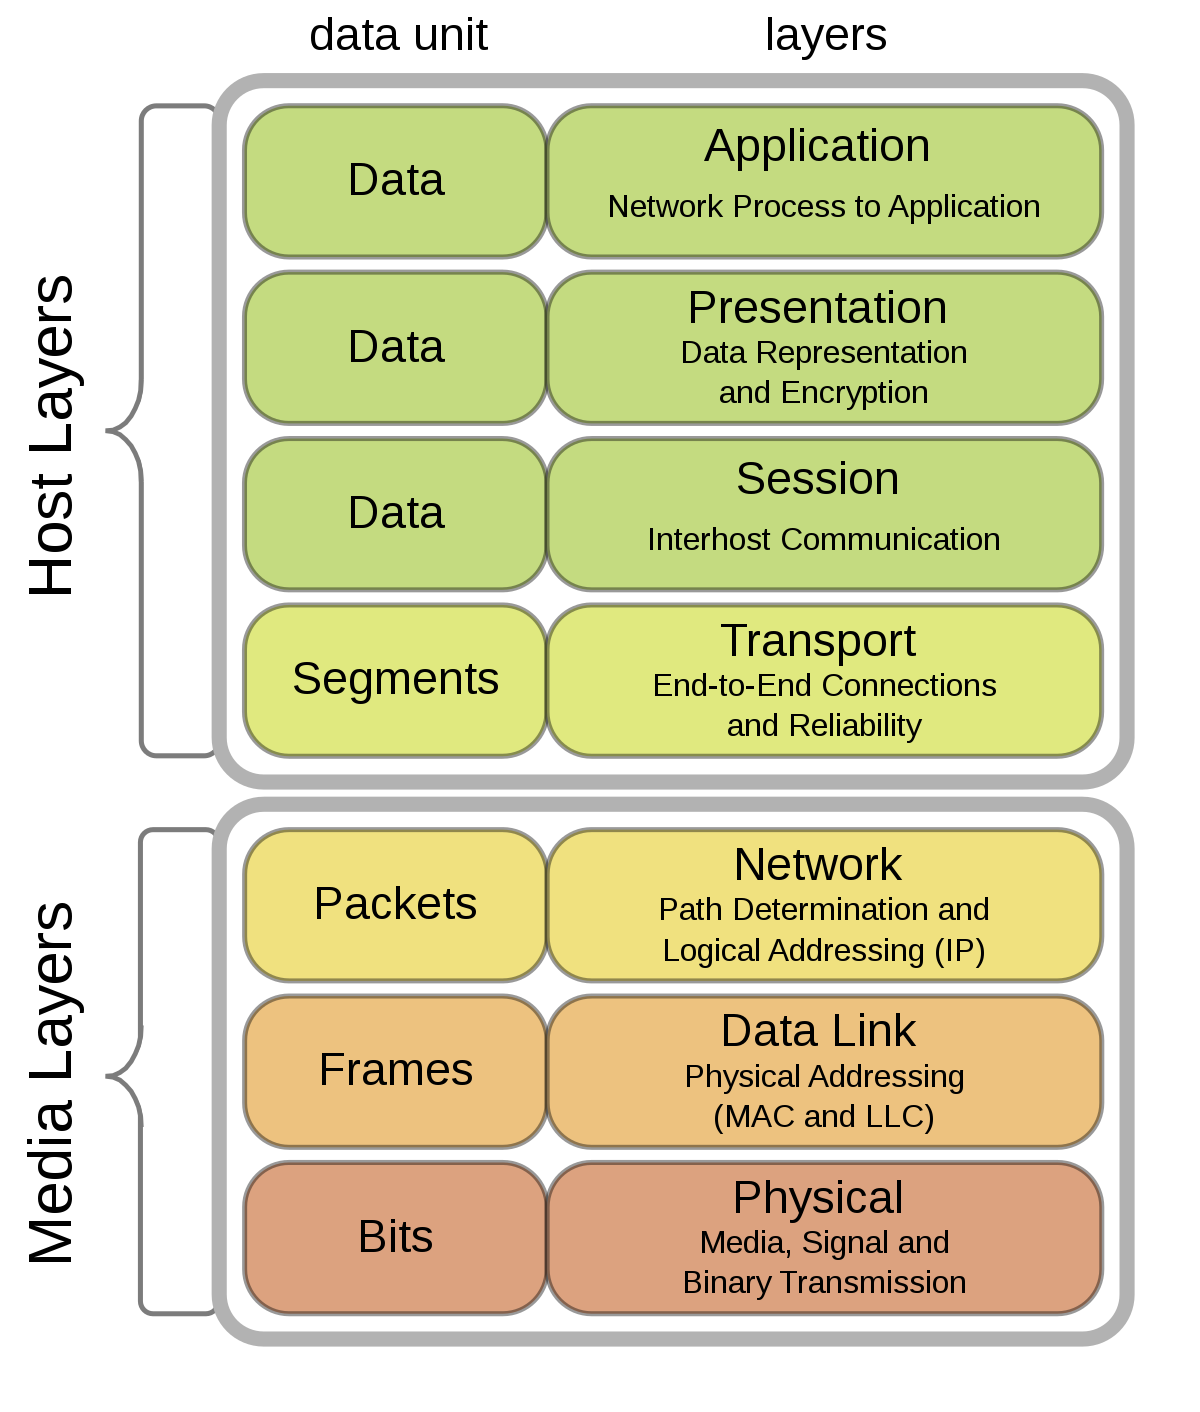
\includegraphics[scale=0.25]{images/OSI.png}
        \end{center}
        
        Ogni strato definisce un insieme di funzioni che si occupano di aspetti diversi della trasmissione dei dati. Più strati possono essere raggrupppati. I processi su due nodi che comunicano a un dato strato sono detti \textbf{peer}.
        
        In particolare, gli strati 1, 2 e 3 (\textit{fisico, collegamento, rete}) sono detti \textbf{Media Layers} e sono dedicati al supporto di rete. Le loro funzionalità hanno a che fare con problematiche del mezzo fisico (specifiche elettriche, connessioni fisiche, indirizzi di rete, sincronizzazione, controllo degli errori).
        
        Invece, gli strati 5, 6 e 7 (\textit{sessione, presentazione, applicazioni}) sono detti \textbf{Host Layers} e sono dedicati al supporto all'utente e permettono l'interoperabilità fra sistemi che usano software diversi fra loro. 
        
        Lo strato 4 (\textit{trasporto}) collega i due gruppi di strati appena descritti, e solitamente viene affibbiato al gruppo di Host Layers.
        
        \vspace{3mm}
        
        Tutti gli strati degli Host Layers sono implementati a livello software, in genere nel sistema operativo. Gli strati dei Media Layers sono ibridi, e cioè implementati a livello sia software che hardware, eccetto che per lo strato fisico, il quale è implementato esclusivamente a livello hardware.
        
        Riprendendo il concetto esposto prima per il quale la flessibilità di un modello si concretizza nella capacità di non usare tutti i layer, si prenda in esame un generico \textit{router}: un dispositivo del genere (talvolta chiamato \textbf{nodo intermedio}), che permette a più sottoreti di interfacciarsi fra di loro, ha necessità solo di uno strato fisico, uno strato di collegamento e uno strato di rete per poter funzionare.
        
        Il modello ISO-OSI è dunque \textbf{modulare}, proprio perché la stratificazione viene impiegata dinamicamente in base alle necessità.
        
        Si osservi che fra due nodi, lo strato \(n\) di un nodo comunica con il corrispondente strato \(n\) di un altro nodo. 
        
        I processi su due nodi che comunicano a un dato strato sono detti \textbf{peer}. Tale comunicazione avviene per mezzo di \textbf{interfacce}. L'implementazione interna dello strato è irrilevante, a patto che fornisca l'esatta interfaccia ad ambo i nodi.
    
    \subsubsection{Trasmissione stratificata dei dati}
    
        \textbf{I dati vengono trasmessi di strato in strato}, a partire da quello più in alto del mittente, per finire in quello più in basso, per poi rientrare dal livello più in basso del destinatario e concludere il suo viaggio al livello più in alto.
        
        \vspace{3mm}
        
        Il passaggio da strato fisico del mittente a strato fisico del destinatario avviene chiaramente tramite un mezzo di comunicazione (bus, hub, cavo, rif. \textit{topologia delle reti}).
        
        \vspace{3mm}
        
        L'utente invia il messaggio tramite lo strato applicativo, magari tramite il Web, un client FTP o qualsiasi altra interfaccia.
        
        \vspace{3mm}
        
        Il viaggio di un pacchetto dati è più o meno sintetizzabile come segue:
        
        \vspace{3mm}
        
        \(>\) Application (Mittente) 
        
        \(>\) [..] 
        
        \(>\) Physical (Mittente) 
        
        \(>\) Physical (Destinatario) 
        
        \(>\) [..] 
        
        \(>\) Application (Destinatario)
        
        \vspace{3mm}
        
        \textbf{Quello che in effetti succede è che ogni strato aggiunge delle informazioni che vengono ereditate dagli strati successivi.}
        
        L'utente invia un dato, un informazione, un messaggio, qualsiasi cosa tramite l'\textbf{Application Layer}. Tale messaggio è indicato come \textit{D7}. Quando è ancora nell'Application Layer, \textit{D7} viene accodato ad un header, cioè un'intestazione contenente svariate informazioni sulla trasmissione dei dati, denotato come \textit{H7}. Il Presentation Layer riceverà un dato del tipo "\textit{H7-D7}". 
        
        \vspace{3mm}
        
        A questo punto, il \textbf{Presentation Layer} accorperà insieme \textit{H7-D7} in un unico, grande, \textit{D6}. Infine, \textit{D6} viene accodato ad un ulteriore header, denotato con \textit{H6}. 
        
        \vspace{3mm}
        
        Il dato \textit{H6-D6} è chiaramente più grande di \textit{H7-D7}. Questo processo viene ripetuto fino allo strato di collegamento. 
        
        \vspace{3mm}
        
        Il \textbf{Data Link Layer}, oltre ad aggiungere il proprio header e accorpare i dati precedenti, piazzerà in coda anche un trailer \textit{T2}, dedicato al controllo degli errori. 
        
        \vspace{3mm}
        
        Il \textbf{Physical Layer}, dunque, riceverà \textit{
        H2-D2-T2}, e il loro contenuto verrà tradotto in binario e trasmesso, tramite un mezzo di comunicazione, al destinatario.
        
        \vspace{3mm}
        
        \textbf{Osserviamo che ad ogni passaggio si ha un pacchetto differente.} Un \textit{pacchetto}, in questo caso, è l'insieme costituito da header, body e trailer.
        
        \vspace{3mm}
        
        Quando il pacchetto arriva nel Phyisical Layer del destinatario, nella sua risalita viene mano a mano smontato. Ogni strato accederà all'header, leggerà delle informazioni, rimuoverà l'headear e scorporerà il body per recuperare l'header successivo. Analogamente per il trailer all'accesso al Data Link Layer.
        
        \vspace{3mm}
        
        I pacchetti vengono incapsulati senza conoscere alcuna informazione relativa all'header dello strato superiore. Il livello \(n-1\) non sa assolutamente niente dell'intestazione del livello \(n\), ma considera tutto il blocco come una singola unità di dati. L'accorpamento descritto fino ad ora è, difatto, \textbf{un passaggio implicito e automatico}.
    
    \subsubsection{Sintesi del funzionamento degli strati}
    
        Questa sottosezione vuole solo elencare in modo molto sintetico le funzionalità principale degli strati del modello ISO-OSI. Per maggiori dettagli, consultare la rispettiva sezione in questo blocco di appunti.
    
        \subsubsubsection{Physical Layer}
        
            Lo \textit{strato fisico} si preoccupa di trasmettere i singoli bit sul mezzo trasmissivo da un nodo ad un altro. Questo significa che lo strato fisico controlla le funzioni richieste per convertire una sequenza di bit negli opportuni segnali da spedire sul mezzo di collegamento. 
            
            \vspace{3mm}
            
            In particolare, lo strato fisico definisce la velocità con cui i segnali vanno spediti; in che modo i bit devono essere sincronizzati per essere letti correttamente dal destinatario; come vanno rappresentati i bit e codificati in segnali; come definire il tipo di mezzo trasmissivo impiegato; di che tipo è la comunicazione (simplex, half-duplex, duplex); di che tipo è la topologia della rete; com'è configurato il collegamento fra i nodi (punto-punto, multipunto).
        
        \subsubsubsection{Data Link Layer}
        
            Lo \textit{strato di collegamento} si occupa della trasmissione affidabile di pacchetti di dati fra un nodo ed il successivo. 
            
            \vspace{3mm}
            
            Per svolgere questo compito, lo strato di collegamento ha molteplici responsabilità: \textbf{framing} (dividere il flusso di bit che arriva dallo strato inferiore in frame da essere spediti allo strato superiore), indirizzi fisici (aggiungere un'intestazione contenente l'indirizzo fisico del destinatario), controllo del flusso (meccanismi per evitare il sovraccarico nel caso in cui il destinatario può ricevere i bit solo a velocità minore rispetto alla velocità del mittente), controllo degli errori (frame duplicati, frame danneggiati), controllo dell'accesso multiplo (nel caso di collegamenti multipunto, lo strato controlla quale nodo ha accesso al mezzo di trasmissione) e così via.
            
            \vspace{3mm}
            
            Lo strato di collegamento usa gli \textbf{indirizzi fisici} (MAC) delle interfacce di rete per far comunicare due nodi sulla stessa rete.
            
            \vspace{3mm}
            
            La \textit{consegna dei frame}, detta \textbf{hop}, avviene fra due nodi successivi. Tale consegna può essere diretta o indiretta. Nel caso di una consegna indiretta, e cioè a più passaggi, i frame conterranno gli stessi dati, ma headers e trailers varieranno per ogni spedizione. 
            
            La consegna indiretta avviene quando la comunicazione dev'essere stabilita fra nodi su reti diverse. Si noti, infine, che la consegna indiretta è concettualmente una sequenza di consegne dirette.
        
        \subsubsubsection{Network Layer}
        
            Lo \textit{strato di rete} si occupa della consegna di pacchetti da un \textbf{nodo mittente} ad un \textbf{nodo destinatario}, attraversando uno o più nodi intermedi. 
            
            Se due nodi sono sulla stessa rete, non avranno bisogno dello strato di rete per comunicare; altresì, fintanto che è necessario instradare il percorso del pacchetto da un nodo A ad un nodo B tramite dei router, allora lo strato di rete è indispensabile.
            
            \vspace{3mm}
            
            Se per raggiungere la destinazione si devono attraversare più nodi, si parla di \textit{consegna indiretta}.
            
            \vspace{3mm}
            
            Questo strato utilizza gli \textbf{indirizzi logici} (IP), composto da 32 bit e rappresentato in notazione decimale puntata, per identificare i nodi da raggiungere. 
            
            Ciò significa che, mentre nello strato di collegamento si ha a che fare con un indirizzamento fisico, nello strato di rete si affronta, invece, un indirizzamento puramente logico, e cioè che non dipende da alcuna componente fisica.
            
            \vspace{3mm}
            
            Il compito principale dello strato di rete è il \textbf{routing} (instradamento). Quando più reti sono connesse fra di loro per creare una interrete, i nodi che intercorrono fra le singole reti (e cioè i nodi intermedi, dunque i router) hanno il compito, appunto, di instradare i pacchetti verso la destinazione finale. 
            
            \textbf{Il pacchetto originale viene suddiviso in pacchetti più piccoli}, detti \textit{segmenti}, che possono seguire percorsi diversi. Al raggiungimento del nodo destinataro, il pacchetto viene riassemblato.
        
        \subsubsubsection{Transport Layer}
        
            Formalmente, lo \textit{strato di trasporto} si occupa della consegna di un messaggio da un processo mittente ad un processo destinatario. 
            
            \vspace{3mm}
            
            Si ponga il caso di avere aperti sul proprio computer Microsoft Teams, Google Chrome e Telegram. Quando mi connetto ad una conferenza su Teams sto chiaramente inviando e ricevendo costantemente dati relativi alle immagini, al suono e via dicendo. Ma quando questi dati arrivano, come fanno a capire che devono essere relazionati ed associati a Teams e non, ad esempio, Chrome? Sia Teams che Chrome condividono lo stesso canale di comunicazione (la propria rete), ma i dati che invio e ricevo tramite Teams devono finire su Teams, e non su Chrome o qualsiasi altro applicativo che usa la mia connedssione.
            
            \vspace{3mm}
            
            In effetti, lo stato di trasporto si occupa proprio di determinare il programma (inteso come processo) al quale devono essere effettivamente inviati i pacchetti dati. L'informazione che mi permette di capire a quale proceso inviare i dati è la porta di rete (es. localhost:\textit{8080}), motivo per cui è necessario aggiungere un ulteriore tipo di indirizzamento, contenuto nell'intestazione pervenuta dallo stato di sessione.
            
            \vspace{3mm}
            
            Questo indirizzamento è chiamato \textbf{indirizzamento dei processi} ed è rappresentato dai numeri di porta.
            
            \vspace{3mm}
            
            Inoltre, lo stato di trasporto si occupa della segmentazione del riassemblaggio dei pacchetti, e del controllo della connessione. Lo stato di trasporto, infatti, offre un servizio che può essere con o senza connessione. 
            
            In una \textbf{comunicazione senza connessione}, i dati vengono spediti in pacchetti indipendenti l'uno dall'altro; invece, in una \textbf{comunicazione con connessione}, lo strato di trasporto del mittente crea una connessione con lo stato di trasporto del destinatario prima di trasferire pacchetti contenenti i dati veri e propri. Inoltre, fra i due vi è la differenza che, rispettivamente, i pacchetti eseguono lo stesso percorso, ed eseguono percorsi differenti.
            
            Infine, lo stato di trasporto controlla, fra i processi terminali (mittente e destinatario), la velocità di trasmissione dei dati, nonché eventuali errori nell'intero processo. Questa caratteristica dello strato di trasporto è denominata "controllo del flusso".
        
        \subsubsubsection{Session Layer}
        
            Lo \textit{strato di sessione} si occupa del controllo di dialogo e della sincronizzazione. Stabilisce, mantiene e sincronizza l'interazione fra i sistemi che comunicano. Questo strato, seppur concettualmente semplice, è fondamentale: permette, infatti, a due sistemi \textit{\textbf{diversi}} di comunicare.
        
        \subsubsubsection{Presentation Layer}
        
            Lo \textit{strato di presentazione} si occupa della sintassi e della semantica dell'informazione trasmessa, dunque cifratura, compressione e traduzione di dati in bit da trasmettere.
        
        \subsubsubsection{Application Layer}
        
            Lo \textit{strato di applicazione} fornisce i servizi di rete all'utente finale. Servizi di posta, World Wide Web, accesso a file remoti, gestione condivisa di database e tanto altro.
            
    \subsection{Accenni alla Suite TCP/IP}
        L'ISO-OSI è un modello di riferimento, nel senso che si suppone che i produttori di hardware e software seguino gli standard proposti per sviluppare i propri servizi. La \textbf{suite TCP/IP} è stata sviluppata quando il modello OSI non era ancora diventato uno standard, motivo per cui sorgono delle disambiguità fra i due. 
    
        \begin{center}
            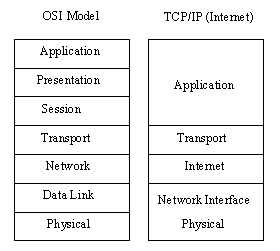
\includegraphics{images/TCP.png}
        \end{center}
    
        La suite TCP/IP permette il funzionamento di Internet. Si ispira all'ISO-OSI e ha una stratificazione a livelli. Ha 5 strati (4 se si accorpano lo strato fisico e quello di collegamento). Il TCP/IP non specifica, né per lo strato fisico, né per lo strato di collegamento, alcun protocollo. Si può usare qualsiasi protocollo previsto dall'hardware di rete. 
    
    \subsubsection{Funzionamento e tipi di indirizzamento}
        Il protocollo che adempie alle funzionalità dello strato di rete è l'\textbf{Internet Protocol} (IP), che usa l'indirizzamento logico per la consegna di pacchetti da un nodo all'altro (datagram). Lo strato di rete non permette una consegna affidabile dei dati perché i datagram possono seguire strade diverse e quindi arrivare alla destinazione in ordine diverso da quello di spedizione, o addiritura duplicarsi o venire persi. Questo servizio di consegna è chiamato "\textit{best-effort}".
        L'IP "\textit{fa del suo meglio}", senza però offrire garanzia alcuna. Ulteriori protocolli utilizzati nello strato di rete sono \textit{ARP} e \textit{RARP} (risoluzone indirizzi), \textit{ICMP} (gestione degli errori) e \textit{IGMP} (trasmissione simultanea).
    
        \vspace{3mm}
    
        Lo stato di trasporto utilizza i protocolli \textit{UDP} (senza garanzie di consegna, implementata per necessità di celerità), \textit{TCP} (trasmissione affidabile) e \textit{SCTP} (per dati multimediali). L'UDP viene adoperato, ad esempio, per gli streaming su Teams: perdere un pacchetto in una conferenza non è chissà che problema, ma perdere un pacchetto durante una transazione bancaria lo è eccome. Per la transazione bancaria verrebbe utilizzato il TCP.
    
        \vspace{3mm}
    
        Lo strato applicativo, che include gli strati di presentazione e di sessione, si rifa in toto all'ISO-OSI. I "protocolli" in questo caso coincidono con i "programmi" utilizzati (posta elettronica, Web, etc).
    
        \vspace{3mm}
    
        \begin{center}
            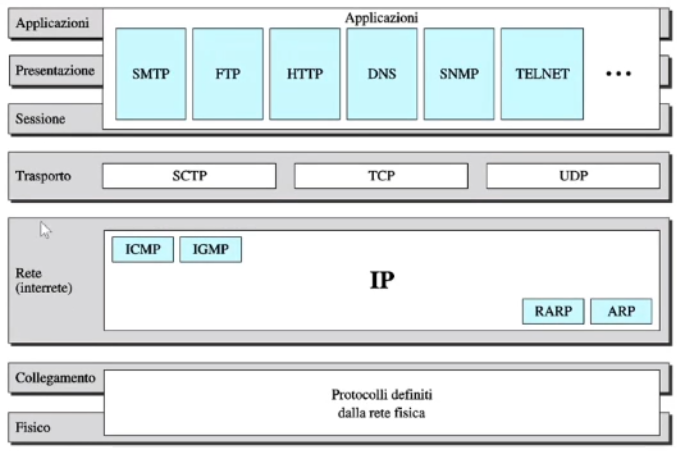
\includegraphics[scale=0.5]{images/TCP-Synth.png}
        \end{center}
    
        \vspace{3mm}
    
        Nella suite TCP/IP vengono impiegati quattro tipi di indirizzamento:
    
        \begin{itemize}
            \item 
                \textbf{Indirizzi fisici} (strato fisico e di collegamento), rappresentato dal MAC Address. E' cablato all'interno della scheda di rete, è una sequenza di 6 byte trascritti nell'interfaccia di rete.
            
            \item
                \textbf{Indirizzi logici} (strato di rete), rappresentato dall'IP Address. E' una sequenza di 4 byte in notazione decimale puntata. Ogni computer connesso ad Internet ha un indirizzo IP.
            
            \item
                \textbf{Indirizzi di porta} (strato di trasporto), rappresentato dai numeri di porta. Gli indirizzi IP e MAC sono necessari per far arrivare i dati al destinatario; tuttavia, su un singolo computer possono essere in esecuzione contemporaneamente più programmi: l'indirizzo di porta ci permette di determinare a quale programma inviare i dati. Le porte sono a 2 byte.
            
            \item
                \textbf{Indirizzi specifici} (strati applicativi), rappresentati da vari indirizzi, come l'indirizzo email.
        \end{itemize}

        Le porte più note sono la porta SSH (22) e la porta dei web server (80).

\section{Rappresentazione di dati e segnali}

    \subsection{Segnali semplici e composti}
    
        La funzione principale dello \textit{strato fisico} è trasportare i dati in forma di \textbf{segnali elettromagnetici} su un mezzo trasmissivo. Questo significa che, per essere trasmessi, i dati devono essere prima trasformati in segnali elettromagnetici.
        
        \vspace{3mm}
        
        \textbf{Esistono due tipi di dati: analogici e digitali.} I \textbf{dati analogici} sono informazioni (valori) rappresentate in forma continua (e cioè il cui dominio è un insieme infinito di possibili valori); invece, i \textbf{dati digitali} sono informazioni (valori) rappresentate in forma discreta (e cioè il cui dominio è un insieme finito di possibili valori, rappresentati con sequenze di 0 e 1).
        
        \vspace{3mm}
        
        \textbf{Esistono due tipi di segnali: analogici e digitali.} I \textbf{segnali analogici} possono assumere un infinito numero di valori in un dato intervallo; invece, i \textbf{segnali digitali} possono assumere solo un numero finito di valori in un dato intervallo.
        
        \begin{center}
            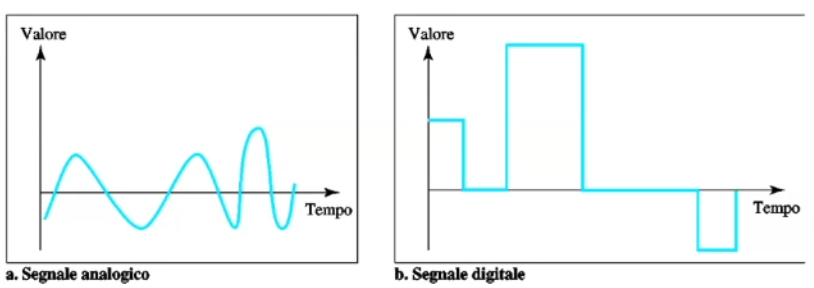
\includegraphics[scale=0.25]{images/Esempio-Segnali.png}
         \end{center}
        
        \vspace{3mm}
        
        Sia i segnali analogici che digitali possono assumere due forme: \textbf{periodica} (varia regolarmente nel tempo) e \textbf{aperiodica} (varia senza regolarità nel tempo).
        
        \vspace{3mm}
        
        In particolare, se un segnale digitale ha \(L\) livelli, ogni livello può facilmente rappresentare \(log_2 L\) bit. La lunghezza di tali bit è l'analogo della lunghezza d'onda per i segnali analogici. Può essere interpretata come la distanza (o lo spazio) che la rappresentazione di un bit occupa sul mezzo trasmissivo. E' funzione di velocità di propagazione e rappresentazione utilizzata. La lunghezza di 1 bit equivale a \((\text{velocità di propagazione})*(\text{durata di 1 bit})\).
        
        Osserviamo che il concetto di livello è escluso dei segnali digitali.
        
        \begin{center}
            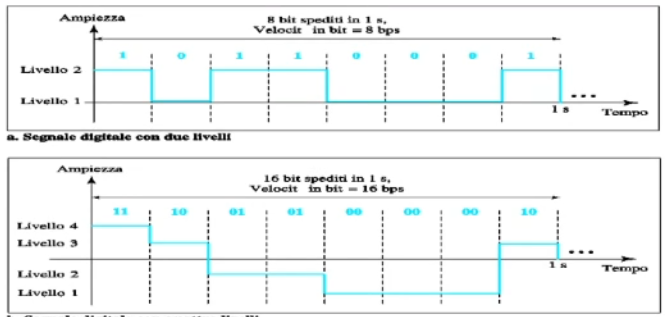
\includegraphics[scale=0.45]{images/Segnali-Digitali-Esempio.png}
        \end{center}
        
        \vspace{3mm}
        
        Per le reti di comunicazione, normalmente vengono usati segnali analogici periodici e segnali digitali non periodici. I primi richiedono minore larghezza di banda e possono essere semplici o composti. I secondi possono rappresentare facilmente i dati.
    
    \subsection{Descrizione delle onde sinusoidali dei segnali analogici}
    
        \subsubsection{Segnali analogici semplici}
    
            \textbf{Un segnale analogico è detto \textit{semplice} se non può essere decomposto in segnali più semplici}, e viene rappresentato graficamente con una curva oscillante (come la funzione \(sen\)). Tale curva dipesa dall'\textit{ampiezza massima} (o di picco; è il valore assoluto del segnale nella sua intensità massima - per segnali elettrici si misura in \textit{volt}), dalla \textit{frequenza} e dalla \textit{fase}.
            
            \vspace{3mm}
            
            Le onde semplici hanno molte applicazioni: ad esempio, sono adatte per il trasporto di energia elettrica, ma sono inadatte per il trasporto di segnali che rappresentano suoni, dati e quindi per le reti di comunicazione in generale.
            
            \vspace{3mm}
            
            Un segnale semplice è descritto tramite:
            
            \begin{itemize}
            
            \item 
                Il \textbf{periodo} è il tempo necessario affinché un segnale completi un ciclo, espresso in \textit{secondi}. Il ciclo è la porzione di curva che si ripete.
            
            \item
                La \textbf{frequenza} è il numero di periodi in 1 secondo, espresso in \textit{hertz}. Può essere interpretata come la velocità con cui il segnale cambia nel tempo, ed è direttamente legata alla velocità di trasmissione.
            
            \item
                Si osservi che il periodo è l'inverso della frequenza, e viceversa.
            
                \begin{center}
                    \(f=\frac{1}{T}\)
                    
                    \(T=\frac{1}{f}\)
                \end{center}
            
            \item
                La \textbf{fase} descrive la posizione dell'onda sinusoidale rispetto al tempo 0, espressa in \textit{gradi} o \textit{radianti}. Se si pensa all'onda come un qualcosa che può essere spostato avanti o indietro lungo l'asse del tempo, la fase descrive l'ampiezza di tale spostamento.
            
                \begin{center}
                    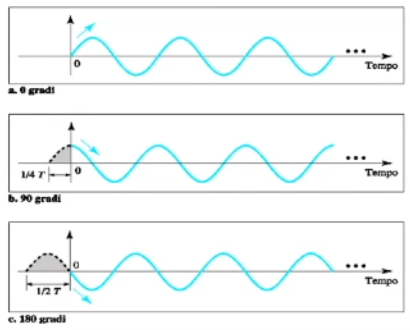
\includegraphics[scale=0.45]{images/Fase.png}
                \end{center}
            
            \item
                La \textbf{lunghezza dell'onda} mette in relazione il periodo \(T\) (o la frequenza \(f\)) con la velocità di propagazione \(c\) del segnale del mezzo. La lunghezza d'onda è funzione del mezzo di trasmissione (oltre che del segnale) e rappresenta la distanza (o meglio lo spazio) che un ciclo del segnale occupa sul mezzo trasmissivo, espressa in \textit{micron}.
            
                \begin{center}
                    \(\lambda=c*T=\frac{c}{f}\)
                \end{center}
            \end{itemize}
            
        \subsubsection{Segnali analogici composti}
        
            Parliamo adesso dei segnali analogici composti. \textbf{Le onde composte sono la somma di onde sinusoidali semplici.} L'\textit{analisi di Fourier} mostra che un qualsiasi segnale composto è la somma di onde semplici con diverse frequenza, ampiezze e fasi.
        
            Un segnale composto è descritto tramite:
            
            \begin{itemize}
                \item
                    Lo \textbf{spettro} è l'insieme delle frequenze di un segnale composto.
                
                \item
                    La \textbf{larghezza di banda} è la differenza fra la frequenza più alta e la più bassa nello spettro.
            \end{itemize}
    
    \subsection{Deterioramento del segnale}
    
        I segnali viaggiano lungo il mezzo trasmissivo, il quale causa un deterioramento del segnale: questo implica che il segnale ricevuto non è esattamente quello inviato. Le cause sono, in genere, l'attenuazione, la distorsione o il rumore del segnale.
        
        \subsubsection{Attenuazione}
        
            L'\textbf{attenuazione} è la perdita di energia subita quando il segnale, viaggiando lungo il mezzo trasmissivo, deve superare la resistenza del suddetto. Questo è anche il motivo per cui il filo elettrico si riscalda quando viene attraversato dal segnale: parte dell'energia elettrica, infatti, viene convertita in calore. 
            
            In termini pratici, man mano che il segnale viaggia si subisce una perdita di energia poiché il mezzo trasmissivo, per sua natura, è dotato di una resistenza che attenua il passaggio del segnale stesso, provocando un fenomeno di perdita di energia, per l'appunto - tale perdita di energia viene trasformata in calore, determinando il surriscaldamento del mezzo trasmissivo.
            
            La perdita di energia è espressa in decibel, che misurano la potenza \textit{relativa} di due segnali (o dello stesso segnale) in due punti differenti. 
            
            \(dB = 10*log_10 \frac{P_2}{P_1}\)
            
            Per ripristinare il valore corretto di decibel viene generalmente posto un \textit{amplificatore} nei pressi del nodo destinatario.
        
        \subsubsection{Distorsione}
        
            La \textbf{distorsione} è il cambiamento della forza del segnale, molto tipica dei segnali composti costituito da varie frequenze. Ogni componente (frequenza) del segnale ha una propria velocità di propagazione lungo il mezzo trasmissivo, il che causa un ritardo per l'arrivo della destinazione.
            
            In particolare, se guardiamo un segnale composto come un insieme di segnali semplici, allora successivamente al viaggio individuale di questi segnali lungo il mezzo trasmissivo, può risultare che il loro arrivo non sia sincronizzato, producendo un segnale composto finale diverso da quello desiderato. I segnali arrivano non allineati, ma risulta distorto, poiché non coincide con quello spedito.
        
        \subsubsection{Rumore}
        
            Il \textbf{rumore} è dovuto ad interferenze esterne. Può essere termico (causato dal movimento casuale degli elettroni nel mezzo trasmissivo), indotto (causato da sorgenti come motori o altri dispositivi esterni), ad impulsi (causato da fonti esterne come fulmini, che causano un repentino cambio del segnale) o ad interferenze (causato dall'eccessiva vicinanza fra due cavi che trasmettono segnali).
    
    \subsection{Velocità di trasferimento}
    
        Per trovare il limite teorico alla velocità in bit occorre conoscere il rapporto fra la potenza del segnale e la potenza del rumore del canale. Ricordiamo che il mezzo trasmissivo, per sua natura, è dotato di rumore.
    
        \begin{center}
            \(SNR[Signal-toNoise-Ratio] = \frac{potenza\ \ segnale}{potenza\ \ rumore}\)
            
            \vspace{3mm}
            
            \(SNR_{db} = 10 log_{10} SNR\)
        \end{center}
        
        La velocità di trasferimento dei bit dipesa dalla larghezza di banda, dal numero di livelli del segnale e dalla qualità del canale (che induce o meno al rumore). I due risultati teorici per il calcolo della velocità massima su un canale di comunicazione sono forniti dal \textit{Teorema di Nyquist} e dal \textit{Teorema di Shannon}.
        
        I teoremi di Shannon e Nyquist forniscono due risultati in letteratura estremamente validi per ciò che concerne la velocità idealistica ed effettiva della trasmissione di dati.
        
        \subsubsection{Teorema di Nyquist}
        
            \(\text{velocità in bit per secondo}=2*(\text{larghezza di banda})*log_2 L\)
            
            \vspace{3mm}
            
            Questo ideale risultato parte dal presupposto che un canale non sia condizionato dal rumore.
            
            \(L\) è il numero di livelli del segnale che possono essere utilizzati per rappresentare i dati. Aumentando \(L\) si aumenta la velocità. Questo risultato ornisce la velocità teorica massima alla quale possiamo spedire i dati. Chiaramente, non si può aumentare \(L\) a piacere, poiché - da un punto di vista pratica - si ridurrebbe l'affidabilità della trasmissione, aumentendo la probabilità di riscontrare errori: questo perchè, all'aumentare della capienza del canale, è più probabile commettere errori.
        
        \subsubsection{Teorema di Shannon}
        
            \(\text{capacità}=(\text{larghezza di banda})*log_2 (1+SNR)\)
            
            \vspace{3mm}
            
            \textbf{Nella realtà non esistono canali senza rumore}. Questo teorema fornisce un valido risultato teorico per la capacità (cioè la velocità massima) di un canale in \textit{bps}. Il risultato è in funzione del canale di trasmissione col suo rumore (SNR) e non dei livelli dei canali.
            
            Poiché Shannon considera l'SNR, considera automaticamente anche il rumore del canale.
            
        Nelle applicazioni pratiche, si sfruttano ambo i teoremi. Shannon determina la capacità (cioè la velocità di trasferimento massima), mentre Nyquist determina il numero di livelli necessari per ottenere la velocità massima. Significa utilizzare la formula inversa di Nyquist per ottenere \(L\), che è un risultato pratico molto valido.
            
    \subsection{Prestazioni della rete}    
        
        Per misurare l'efficienza di una rete, in genere, si valutano numerosi parametri. Definiamo le più importanti.
        
        \subsubsection{Larghezza di banda}
        
            Espressa in \textit{hertz}, è la larghezza di banda delle frequenze utilizzate per la trasmissione. E' dunque l'intervallo di frequenze utilizzate dal segnale, o l'insieme di frequenze che possono essere spedite lungo il canale.
            
            Espressa in \textit{bps}, misura la velocità massima alla quale possiamo spedire bit sul canale.
            
        \subsubsection{Throughput}
        
            \textbf{Misura quando velocemente possiamo spedire i dati su una rete.} A differenza della larghezza di banda, è una \textbf{misura effettiva}.
            
        \subsubsection{Latenza}
        
            \textbf{Misura quanto tempo occorre a trasferire un intero messaggio.} In effetti, è il tempo misurato dal primo bit spedito  all'ultimo bit arrivato, e consiste in tempo di trasmissione, di propagazione, di attesa e di inoltro.
            
            \vspace{3mm}
            
            Il tempo di trasmissione misura il tempo per immettere i dati sul mezzo.
            
            \begin{center}
                \(T_T = \frac{\text{dimensione dei dati (in bit)}}{\text{larghezza di banda}}\)
            \end{center}
            
            Il tempo di propagazione misura il tempo necessario al segnale per propagarsi sul mezzo trasmissivo.
            
            \begin{center}
                \(T_P = \frac{\text{distanza}}{\text{velocita' di propagazione del segnale}}\)
            \end{center}
            
            I tempi di attesa e di inoltro riguardano, rispettivamente, l'attesa nei nodi intermedi e il tempo necessario al nodo intermedio per smistare il messaggio.
            
        \subsubsection{Prodotto banda-ritardo}
        
            E' il prodotto \(\text{(larghezza di banda)}*\text{(latenza)}\).
            
            Definisce il numero di bit che servono per riempire il canale.
            
            In termini informali, il prodotto banda-ritardo rappresenta il numero di bit si possono avere lungo il mezzo trasmissivo prima che il primo bit arrivi a destinazione.
            
        \subsubsection{Jitter}
        
            Misura la variabilità del ritardo con cui vari messaggi, cioè i pacchetti, vengono consegnati alla destinazione. E' chiaramente necessario che i pacchetti vengano consegnati con lo stesso ritardo.
\section{Conversione dei segnali}

    Abbiamo visto come sono fatti i dati; i dati devono essere trasformati in segnali elettromagnetici, e questi segnali vanno trasmessi. Quando i dati devono essere trasmessi su un mezzo trasmissivo, devono essere prima convertiti in segnali.
    
    Il tipo di segnale (analogico/digitale) dipende dal mezzo trasmissivo. I tipi di dati (analogico/digitale) dipende da tutt'altri parametri.
    
    Ricordiamo che una rete di comunicazione è progettata per spedire dati da un punto all'altro. I dati devono essere convertiti in segnali analogici o digitali, e sono poi trasportati dal mezzo trasmissivo.
    
    Se la forma originale dei dati è diversa dal tipo di segnale supportato dal canale trasmissivo, può essere necessaria una conversione "dati-segnali".
    
    \begin{itemize}
        \item Analogico - Digitale
        \item Digitale - Analogico
        \item Analogico - Analogico
        \item Digitale - Digitale
    \end{itemize}
    
    Le necessità di convertire i primi due set è ovvia. Tuttavia, anche quando i dati sono nella stessa forma del segnale trasportabile può essere necessaria una conversione. 
    
    I dati digitali possono essere rappresentati in vari modi da un segnale digitale (codifica di linea); analogamente, un segnale analogico può dover essere modulato su altre frequenze per essere trasmesso su un canale analogico.
    
    \subsection{Conversione digitale-digitale}
    
        Partendo da dati digitale, li si vuole convertire in segnali digitali -- lo si fa perché i mezzi trasmissivi adoperati impongono questo tipo di rappresentazione.
        
        Può risultare ambigua la necessità di dover convertire un dato digitale in un segnale digitale. Questo succede perché l'unità di base dei dati digitali è il bit, nettamente diverso dall'unità di base dei segnali digitali, che sono elementi di voltaggio (voltaggi positivi, nulli, negativi). Si parte dunque dal presupposto che le informazioni siano salvate come bit.
        
        Si parla quindi di una rappresentazione di dati digitali usando segnali digitali. Esistono due grandi categorie di codifica (cioè conversione) digitale-digitale: la \textit{codifica di linea} e la \textit{codifica a blocchi}.
    
        \subsubsection{Codifiche di linea}
        
            La \textbf{codifica di linea} assume che i dati siano memorizzati nella memoria del computer come sequenze di bit. La codifica in sé permette di convertire una sequenza di bit in segnali digitali.
            
            Il mittente esegue la conversione binaria dei dati, e il destinatario ricostruisce i dati digitali dal segnale digitale. In questa tecnica risultano necessari un codificatore e un decodificatore. 
            
            \vspace{3mm}
            
            In generale, con \textit{elemento dei dati} si intendono i bit 0/1, ossia il più piccolo pezzo di informazione che si può rappresentare; l'\textit{elemento del segnale}, invece, è il più piccolo elemento del segnale che possiamo utilizzare. Il rapporto $r$ è il numero di bit rappresentati da un elemento del segnale.
            
            \vspace{3mm}
            
            E' possibile caratterizzare la codifica di linea come segue.
            
            \begin{itemize}
                \item \textbf{Unità di base dei dati e dei segnali.} Si distinguono gli elementi dei dati, intesi come i bit, e gli elementi del segnale, e si valuta il loro rapporto, che corrisponde al numero di bit rappresentati da un elemento del segnale.
                
                \item \textbf{Velocità dei dati e velocità del segnale.} La velocità dei dati $N$ è il numero di bit spedibili in 1 $s$ ($bps$). La velocità degli elementi del segnale $S$ è il numero di elementi di segnale spedibili in 1 $s$ ($baud$). 
                
                La formula per calcolare $S$ sarà \(S=c*n*\frac{1}/r baud\), dove $c$ è un fattore che dipende dal caso considerato. Osserviamo che la velocità del segnale dipesa dalla velocità dei dati.
                
                \item \textbf{Linea di base.} Nella codifica di un segnale digitale, il destinatario calcola in tempo reale la media della potenza del segnale che riceve (\textit{linea di base}). Il segnale ricevuto viene confrontato con la linea di base per determinare il valore dell'elemento del segnale che si deve decodifcare. Lunghe sequenze di valori uguali falsano la media.
                
                In termini semplici, la linea di base rappresenta il valore medio della potenza utilizzato dal destinatario per capire come interpretare i bit in arrivo.
                
                \item \textbf{Componenti DC (Direct Current).} Quando il voltaggio di un segnale è costante per un certo periodo di tempo vengono utilizzate frequenze molto basse, vicine allo zero. Risulta un problema, poiché' su alcuni collegamenti non è è possibile il passaggio di frequenze basse.
                
                \item \textbf{Sincronizzazione automatica.} Per interpretare correttamente la lettura del segnale da parte del destinatario, deve corrispopndere agli intervalli di tempo usati dal mittente per generare il sdegnale. I clock possono non essere perfettamente sincronizzati, quindi serve introdurre degli elementi di sincronizzazione.
            \end{itemize}
            
            Gli schemi di codifica di linea sono schemi che permettono la rappresentazione dei dati (bit) con elementi del segnale digitale. I più utilizzati in letteratura sono l'\textbf{unipolare} (NRZ), il \textbf{polare} (NRZ, RZ e bifase), il \textbf{bipolare} (AMI e pseudoternaria), il \textbf{multilivello} (2B/1Q, 8B/6T, 4D-PAM5) e il \textbf{multilinea} (MLT-3). 
            
            Il problema di passare da uno schema all'altro riguarda la sincronizzazione, e cioè legato alla capacità di decodifica del messaggio da parte del destinatario, il quale riceve un segnale digitale e deve imparare a fissare un clock di sincronizzazione che gli permettere di suddividere e decodificare tale segnale digitale.
            
            \vspace{3mm}
            
            La codifica di linea è dunque definibile come la rappresentazione, intesa come i livelli di voltaggio (unipolare, bipolare, etc) e la loro organizzazione, che andiamo ad utilizzare per fornire informazioni di sincronizzazione.
        
            \vspace{3mm}
        
            In sintesi, gli schemi di codifica ci dicono come si rappresenta un bit rispetto ad un altro.
        
        \subsubsection{Codifica NRZ}
        
            In uno schema unipolare, che è il più semplice, i valori di tutti i livelli del segnale che vengono utilizzati hanno lo stesso segno (tutti positivi o nulli, tutti negativi o nulli), e viene detto \textbf{Non-Return-to-Zero} (NRZ). 1 rappresenta un voltaggio positivo, 0 un voltaggio zero.
            
            Nell'esempio seguente, si è scelto di rappresentare il bit 1 con voltaggio positivo, e il bit 0 con voltaggio negativo.
            
            \begin{center}          
                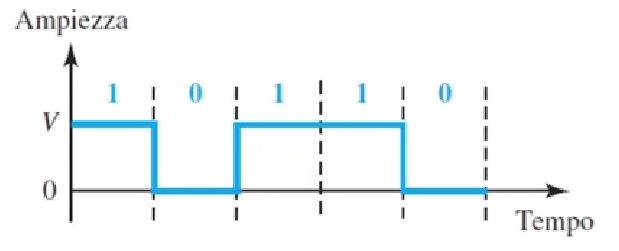
\includegraphics[scale=0.5]{images/NRZ.png}
            \end{center}
            
            Lo schema NRZ è stato poi esteso negli schemi polari per dare più informazioni sull'andamento del segnale, e cioè sulla variabilità del segnale rispetto alla rappresentazione.
            
            \vspace{3mm}
            
            Nel NRZ-L (Level), il livello del voltaggio determina il valore dei bit.
            
            Nel NRZ-I (Inverted), il valore dei bit è determinato dall'assenza o presenza di un cambio di livello del voltaggio.
            
            \begin{center}
                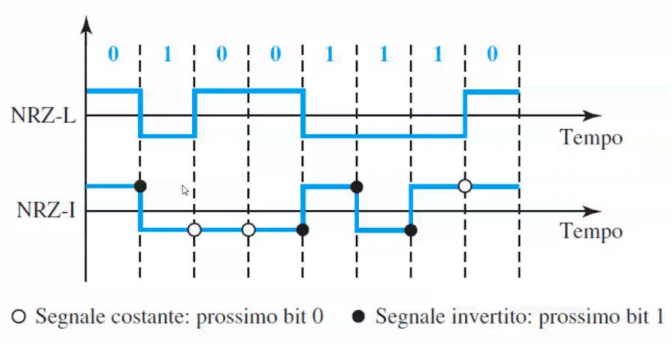
\includegraphics[scale=0.5]{images/NRZ-LeI.png}
            \end{center}
        
            Il problema principale degli schemi polari è, ad esempio, che nella codifica NRZ-L, se c'è una sequenza lunga di 0 o 1, il valore medio della potenza del segnale si avvicinerà sempre più al valore del voltaggio positivo (o negativo) che rappresenta 0 o 1. 
            
            Il destinatario potrebbe dunque avere problemi a distinguere una tensione positiva o negativa da un'assenza di tensione. Vi è inoltre il problema della sincronizzazione dei clock fra mittente e destinatario, e dei componenti DC. Indubbiamente, il problema più accentuato negli schemi NRZ è quello della sincronizzazione.
        
        \subsubsection{Codifica RZ}
        
            La codifica RZ risolve il problema della sincronizzazione. Utilizza 3 livelli di segnale, cioè positivo, negativo e zero, e il valore 0 rappresenta una tensione negativa, mentre il valore 1 una tensione positiva. Il segnale torna sempre a zero al centro di ogni bit e rimane su tale valore fino all'inizio del prossimo bit.
            
            Nella pratica, nel RZ si parte da un elemento di segnale negativo o positivo, e si impone che si ritorni - a prescindere - sempre ad una posizione centrale, cioè nulla.
            
            \begin{center}
                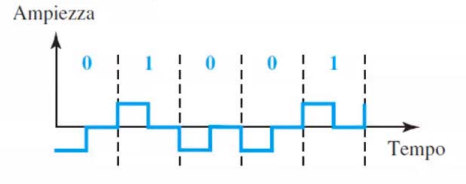
\includegraphics[scale=0.5]{images/RZ.png}
            \end{center}
        
        \subsubsection{Codifiche Manchesters}
        
            L'idea della transizione al centro di ogni bit (RZ) combinata con la codifica NRZ-L produce la codifica \textbf{Manchester}. Ogni singolo bit viene rappresentato da due elementi del segnale, e il valore del bit è determinato dal voltaggio usato, che sarà sempre diverso (ad esempio, il bit 0 è rappresentanto da un voltaggio positivo e uno secondo negativo). 
            
            La combinazione fra NRZ-I e RZ produce, invece, la codifica \textbf{Manchester differenziale}, dove ogni singolo bit viene rappresentato da due elementi del segnale, e il suo valore è determinato dall'assenza o presenza di una transizione all'inizio dell'intervallo.
            
            Nella codifica bifase (come le Manchesters), la transizione al centro viene usata per la sincronizzazione dei clock. La velocità richiesta è due volte quella richiesta dale codifiche NRZ.
            
            \begin{center}
                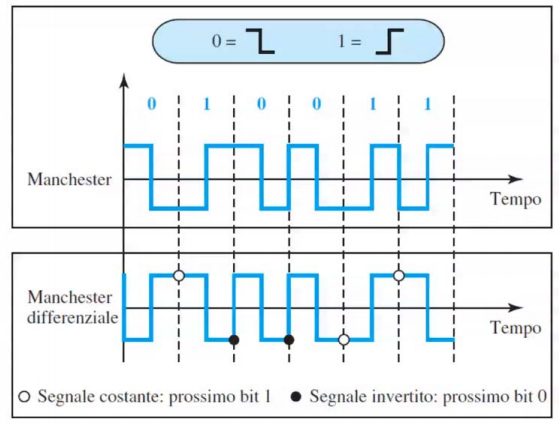
\includegraphics[scale=0.5]{images/Manchesters.png}
            \end{center}
            
            Il vantaggio dell'integrazione RZ con le tecniche bipolari giace nella sincronizzazione. La capacità di rappresentare un bit con due elementi di segnali significa fornire un'informazione di clock aggiuntiva al destinatario. 
            
            La velocità richiesta è circa due volte quella richiesta dagli schemi NRZ.
        
        \subsubsection{Codifiche bipolari, AMI, pseudoternarie e multilivello}
        
            La codifica bipolare risolve ulteriormente il problema della sincronizzazione.
        
            Nella \textbf{codifica bipolare}, vengono utilizzati 3 livelli del segnale: positivo, negativo e zero. Il valore di un bit viene rappresdentato o da un voltaggio pari a zero o da un voltaggio diverso da zero. Richiede la stessa velocità di segnale, ma non componenti DC. Per lunghe sequenze di 0, il vantaggio è costante. 
            
            La codifica NRZ concentra la maggior parte dell'energia vicino alla frequenza nulla, e quindi non è adatta a canali che hanno cattive prestazioni per questo tipo di frequenze, mentre gli schemi bipolari concentrano l'energia attorno alla frequenza N/2.
            
            \vspace{3mm}
            
            La codifica \textbf{AMI} (Alternate Mark Inversion) rappresenta con 0 il voltaggio nullo, 1 voltaggi positivi e negativi che si alternano, ed è utilizzata per le comunicazioni a grande distanza. La \textbf{codifica pseudoternaria} utilizza la rappresentazione opposta.
            
            \vspace{3mm}
            
            In ogni caso, si ha la necessità di aumentare la velocità dei dati. Le \textbf{codifiche multilivello} hanno l'obiettivo di incrementare il numero di bit spediti in media per ogni elemento di segnale codificando una sequenza di \(m\) bit con una sequenza di n elementi del segnale. Sono solitamente indicate con sigle \(mBnL\), dove m è la lunghezza della sequenza dei dati, B indica che i dati sono binari, \(n\) è la lunghezza della sequenza del segnale, e L indica il numero di livelli.
            
            \vspace{3mm}
            
            In particolare, la \textbf{codifica multilivello 2B1Q} rappresenta 2 bit con un elemento di segnale a 4 livelli, e cioè ad una velocità doppia rispetto al NRZ-L.
        
        \subsubsection{Codifiche a blocchi}
            
            Come sempre, la codifica a blocchi risolve ancora di più il problema di sincronizzazione, cioè come "spezzare" il segnale per carpirne i bit.
            
            Oltre alla codifica di linea, è emersa nel tempo la codifica a blocchi. Per ottenere la sincronizzazione dei clock, occorre introdurre il concetto di ridondanza. 
                
            Se nella codifica di linea, le informazioni di sincronizzazione devono essere interpretate da come il segnale è rappresentato, nella codifica a blocchi si interviene al momento dell'invio del messaggio introducendo dei bit ridondanti, che ci permettono di capire quando terminare l'analisi di una parola.
                
            La codifica a blocchi viene solitamente chiamata codifica \(mB/nB\), perchè trasforma una parola sorgente di \(m\) bit in una parola di \(n\) bit con \(n>m\). 
                
            Ad esempio, La \textbf{codifica a blocchi 4B/5B} è sincronizzabile e non produce mai una sequenza con più di 3 zero consecutivi.
                
            \vspace{3mm}
                
            In genere, \textbf{vengono usate sia codifiche di linea} (per rappresentare i dati), \textbf{sia codifiche a blocchi} (per ottenere la sincronizzazione).
            
            \begin{center}
                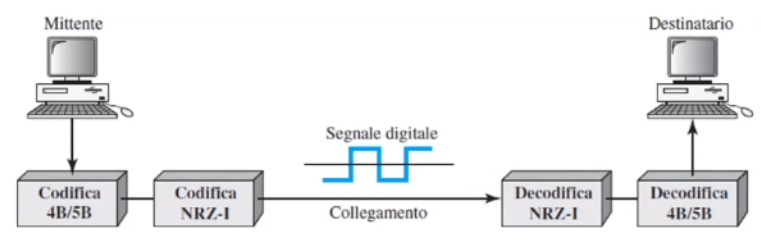
\includegraphics[scale=0.45]{images/Utilizzo-Codifiche-di-Linea.png}
            \end{center}
            
    \subsection{Conversione analogico-digitale}
    
        Si tratta di trasformare un dato analogico, rappresentato dunque in forma d'onda, in un segnale digitale, e cioè ad elementi del segnale. La tecnica più utilizzata per la codifica analogico-digitale prende il nome di \textit{modulazione a impulsi codificati}.
        
        \subsubsection{Modulazione a impulsi codificati}
        
            La \textbf{modulazione a impulsi codificati} converte un segnale analogico in dati digitali in tre fasi:
            
            \begin{itemize}
                \item 
                    \textbf{Campionamento.} Il segnale analogico viene campionato, e cioè misurato a intervalli regolari. Si terrà conto solo delle misurazioni fatte in questi intervalli. Il risultato sarà un numero di valori discreti.
                   
                    Il segnale analogico viene misurato a intervalli regolari $T_S$ e si stabilisce che ad ogni intervallo $T_S$ il segnale debba essere misurato. La \textbf{frequenza di campionamento} è \(f_S = \frac{1}{T_S}\).
                   
                    Vi sono tre tipi di campionamento: \textbf{ideale} (gli impulsi del segnale sono misurati in istanti di tempo a distanza $T_S$), \textbf{naturale} (la misura del segnale avviene in brevi intervalli che includono l'istante di campionamento), e \textbf{a gradini} (simile alla naturale, ma il risultato della misurazione è costante).
                    
                    \vspace{3mm}
                    
                    Ricordiamo che \textbf{l'obiettivo è avere un certo numero di misurazioni che siano effettivamente rappresentative del segnale}. Ridurre il numero di misurazione potrebbe ledere alla precisione dei dati; al contrario, aumentare eccessivamente il numero di misurazioni causerebbe un forte di ritardo nella costruzione della codifica. Si tratta di un problema di computazione. Bisogna, quindi, trovare una via di mezzo fra una qualità soddisfacente del campionamento e una buona velocità di computazione (codifica). 
                   
                    Per fare questo, si usa un risultato di Nyquist, chiamato il \textbf{Teorema di Campionamento}, che enuncia che la velocità di campionamento $f_S$ deve essere \textit{almeno} due volte la frequenza più alta contenuta nel segnale $f$.
                   
                    \begin{center}
                        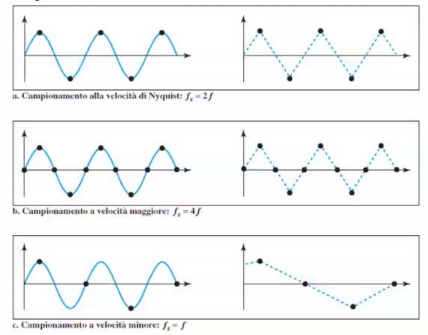
\includegraphics[scale=0.75]{images/Campionamento.png}
                    \end{center}
                
                \item
                    \textbf{Quantizzazione.} Si occupa di rappresentare le misurazioni in termini di \textit{valori}, ossia ricavare dalle misurazioni una quantificazione digitale in bit.
                    
                    Innanzitutto si individua la differenza fra l'ampiezza minima e massima del segnale; dopodichè, si effettua una scelta progettuale: l'intervallo compreso fra l'ampiezza minima e massima del segnale viene diviso in $L$ intervalli d'ampiezza $\delta = \frac{(V_max - V_min)}{L}$. Ciascun intervallo viene rappresentato da un cosiddetto valore di quantizzazione compreso tra $0$ e $L-1$. Infine, ogni misura del campionamento viene approssimata al valore di quantizzazione del corrispondente intervallo.
                
                \item
                    \textbf{Codifica.} Si trasformano i valori di quantizzazione in sequenze di bit. Poiché i valori sono compresi fra $0$ e $L-1$, è sufficiente usare la rappresentazione binaria del valore di quantizzazione. Il numero di bit necessari è $n_b = log_2 L$.
                    
                     La conversione digitale-digitale e analogico-digitale hanno in comune la fase di codifica, ossia l'impiego di un mezzo che richiede una rappresentazione digitale dei dati.
                    
                    La velocità per rappresentare il segnale campionato è $Velocita' dei dati = f_s * n_b$
            \end{itemize}
            
    \subsection{Conversione digitale-analogico}
    
        Trasforma i dati digitali in segnali analogici. \textbf{L'obiettivo è costruire un'onda analogica}, cioè un'onda sinusoidale, che è definita da ampiezza, frequenza e fase. Variando queste caratteristiche, si ottiene una differente onda e quindi dati digitali diversi. Si hanno 4 meccanismi di modulazione: ASK (\textbf{Amplitude Shift Keying}), FSK (\textbf{Frequency Shift Keying}), PSK (\textbf{Pulse Shift Keying}), QAM (\textbf{Quadrature Amplitude Modulation}). L'ultima derivate dalle prime tre.
        
        \vspace{3mm}
        
        \textbf{Dobbiamo costruire tre informazioni} (ampiezza, frequenza e fase), fissando in maniera progettuale 2 di queste dimensioni. Da queste 2, capiamo come costruire la terza. 
        
        \vspace{3mm}
        
        Nell'\textbf{ASK} viene modificata l'ampiezza, quindi frequenza e fase rimangono costanti. Si parla di modulazione binaria (BASK - Binary ASK), utilizza solo 2 livelli e un elemento del segnale può assumere ampiezza massima 1 e minima 0.
        
        \vspace{3mm}
        
        Nel \textbf{FSK} viene modificata la frequenza. Si parla di modulazione binaria (BFSK) e utilizza due frequenze portanti $f_1$ e $f_2$. $f_2$ utilizza valori 0, $f_1$ valori 1.
        
        \vspace{3mm}
        
        Nel \textbf{PSK} viene modificata la fase. E' la più utilizzata. Si parla di modulazione binaria (BPSK), e si hanno due tipi di segnali: uno con fase 0° e uno con fase di 180°.
        
    \subsection{Conversione analogico-analogico}
    
        Si ha necessità di fare questa conversione poiché, ad esempio, una stazione radio deve trasmettere su frequenze diverse, e cioè si ha necessità di convertire un segnale in maniera tale che possa essere trasmesso su una frequenza ammissibile rispetto al canale che stiamo utilizzando. 
        
        Si hanno 3 tecniche: AM (\textbf{Amplitude Modulation}, dove il segnale portante viene modulato in modo tale che l'ampiezza vari al cambiare dell'ampiezza del segnale modulante, mentre frequenza e fase rimangono invariate), FM (\textbf{Frequency Modulation}, dove il segnale portante viene modulato in modo tale che la frequenza vari al cambiare dell'ampiezza del segnale modulante, mentre ampiezza e fase rimangono invariate) e PM (\textbf{Phase Modulation}, dove segnale portante viene modulato in modo tale che l'ampiezza venga rappresentata da variazioni della fase del segnale portante, mentre ampiezza e frequenza rimangono invariate). 
        
        Concettualmente funzionano come la conversione digitale-analogico: si fissano due dimensioni e se ne ricava una terza, definita dal nome della tecnica.
        
    \subsection{Modalità di trasmissione}
                
        Il mezzo trasmissivo può utilizzare, da un punto di vista fisico, uno o più \textit{fili}. Quando trasmettiamo su un mezzo trasmissivo dei dati digitali, si possono avere più modalità di trasmissione: \textbf{trasmissione seriale} e \textbf{trasmissione parallela}. La prima usa un filo e può spedire un solo bit per volta; la seconda usa più fili e può spedire più bit alla volta.
            
        \subsubsection{Trasmissione seriale}
            
            Un solo bit occupa il mezzo trasmissivo. Il vantaggio della \textbf{trasmissione seriale} è il costo ridotto. Lo svantaggio è costituito dalla scarsa velocità. In ogni caso, la trasmissione seriale può essere \textit{sincrona} e \textit{asincrona}. 
                
            \vspace{3mm}
                
            La \textbf{trasmissione seriale asincrona} non da molto importanza alla sincronizzazion; i bit vengono raggruppati in byte, ai quali si aggiungono informazioni intrinseche alla sincronizzazione (bit di start e bit di stop) -- è quindi un meccanismo di ridondanza. Questi bit ci permettono di dire quando inizia e finisce un byte. 
                
            \vspace{3mm}
                
            La \textbf{trasmissione seriale sincrona} raggruppa i flussi di bit in frame, che contiene più byte, e i bit vengono sperditi uno dopo l'altro senza bit di start e di stop, e il destinatario dovrà separare i bit dalla sequenza per ottenere i byte.
            
        \subsubsection{Trasmissione parallela}
            
            La \textbf{trasmissione parallela} organizza il flusso di $n$ bit da spedire su $n$ fili distinti. La spedizione dei bit è contemporanea. Il vantaggio della è la velocità di trasmissione. Lo svantaggio è il costo elevato, motivo per cui la trasmissione parallela viene in genere impegata solo per comunicazioni a breve distanze.
\section{Multiplexing}
    Quando la larghezza di banda di un canale trasmissivo è maggiore della larghezza di banda effettivamente necessaria, il canale può essere condivisdo da più trasmissioni contemporaneamente.
    
    \vspace{3mm}
    
    \textbf{Il multiplexing è definito come l'insieme delle tecniche che permettono la trasmissione simultanea di più segnali su un singolo canale di comunicazione.} Utilizzare canali con una larghezza di banda grande per potere trasportare contemporaneamente dati di più canali logici.
    
    \vspace{3mm}
    
    Ad esempio, si ponga il caso di dover spedire dati a 3Mbps su un canale a 10Mbps: in questo caso, sprecheremmo 7Mbps.
    
    \begin{center}
        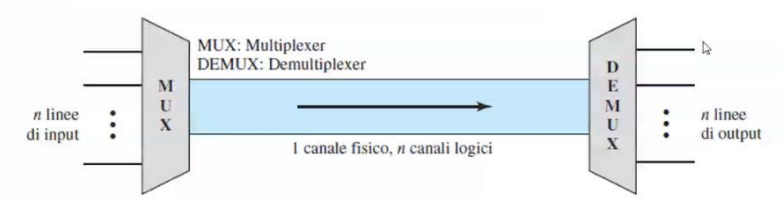
\includegraphics[scale=0.6]{images/Multiplexing.png}
    \end{center}
    
    In un sistema con multiplexing vi è un canale fisico e $n$ linee trasmissive. Per la spedizione occorre aggregare i dati su canali logici e questo lavoro viene svolto dal \textbf{multiplexer} (MUX) che crea un singolo segnale che verrà spedito sul canale fisico; per la ricezione, invece, occorre ridividere i dati aggregati tra i vari canali logici. Il \textbf{demultiplexer} (DEMUX) riconverte il segnale ricevuto nei segnali originali.
    
    \subsection{Tecniche di Multiplexing}
        Esistono tre tecniche generali per implementare il multiplexing.
    
        \begin{itemize}
            \item 
                \textbf{FDM.} E' una tecnica di multiplexing per  segnali analogici. I segnali dei singoli canali logici vengono modulati usando frequenze portanti diverse; i segnali così ottenuti vengono combinati in un singolo segnale composto che può essere trasportato sul collegamento. Le frequenze portanti vengono scelte in modo tale che i segnali modulanti non interferiscano l'uno con l'altro.
                
                \begin{center}
                    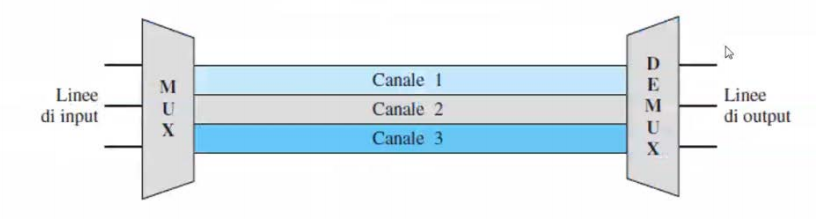
\includegraphics[scale=0.6]{images/FDM.png}
                \end{center}
                
                In fase di \textit{multiplexing}, ogni canale logico genera un segnale sulle stesse frequenze. All'interno del multiplexer questi segnali simili vengono modulati utilizzando segnali portanti di frequenza diversa. I segnali che derivano da ognuna delle modulazioni vengono combinati per creare un singolo segnale composto.
                
                \begin{center}
                    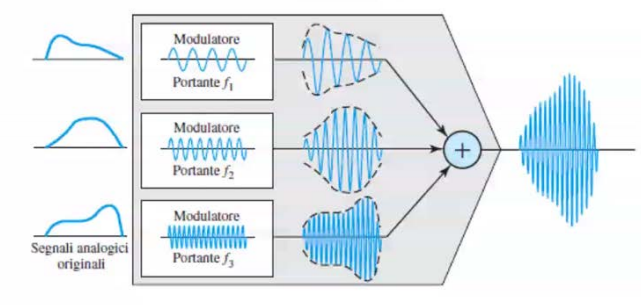
\includegraphics[scale=0.6]{images/FDM_Mult.png}
                \end{center}
                
                In fase di \textit{demultiplexing}, il demultiplexer utilizza una serie di filtri per scomporre il segnale composto ricevuto nei singoli segnali originali. Ciascun segnale viene fatto passare attraverso un demodulatore che supera il segnale che rappresenta i dati originali dal segnale portante usato per modularlo.
            
                \begin{center}
                    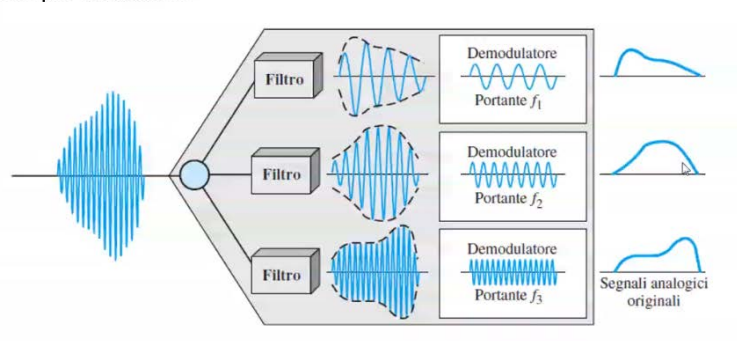
\includegraphics[scale=0.6]{images/FDM_Demult.png}
                \end{center}
            
            \item
                \textbf{WDM.} Tecnica di multiplexing per segnali ottici, utilizza per i cavi in fibra ottica a velocità elevata.
                
                \begin{center}
                    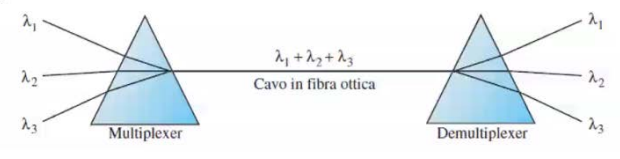
\includegraphics[scale=0.6]{images/WDM.png}
                \end{center}
                
                La modulazione è effettuata sulla lunghezza d'onda del segnale; è una tecnica complessa ma l'idea di base è semplice: si combinano varie sorgenti di luce in un singolo segnale luminoso (multiplexer) o si fa l'esatto opposto (demultiplexer). Le operazioni di raggruppamento e di divisione dei segnal iluminosi possono essere effettuate mediante un prisma, che devia un raggio luminoso in base all'angolo di incidenza e alla frequenza.
             
            \item
                \textbf{TDM.} Progettato per condividere un canale digitale. Invece di condividere una porzione della larghezza di banda, come nel FDM, esso conmdivide il tempo di utilizzo del collegamento. Ogni canale logico occupa un intervallo di tempo in maniera sincrona o statistica.
                
                \begin{center}
                    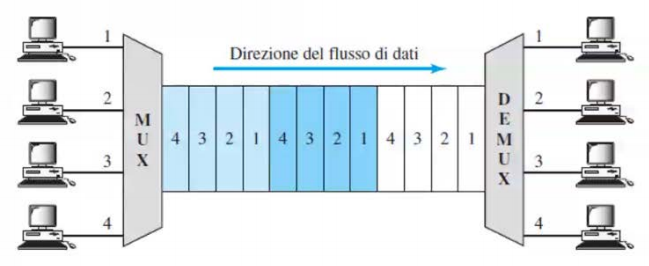
\includegraphics[scale=0.6]{images/TDM.png}
                \end{center}
                
                \begin{itemize}
                    \item 
                        Nel \textbf{TDM sincrono}, l'utilizzo del collegamento fisico viene suddiviso in intervalli di tempo. Il canale viene sfruttato a turno da ogni singolo canale logico. 
                        
                        La grandezza dell'intervallo in sé è un parametro dello schema, che determina il numero di bit che si possono spedire in quell'intervallo. La velocità del collegamento è $n$ volte quella dei canali. 
                        
                        I dati provenienti da ognuno dei canali vengono spediti a turno, seguendo un ordine prestabilito. Gli intervalli sono assegnati staticamente; se un canale non ha dati, l'intervallo viene sprecato.
                    
                        \begin{center}
                            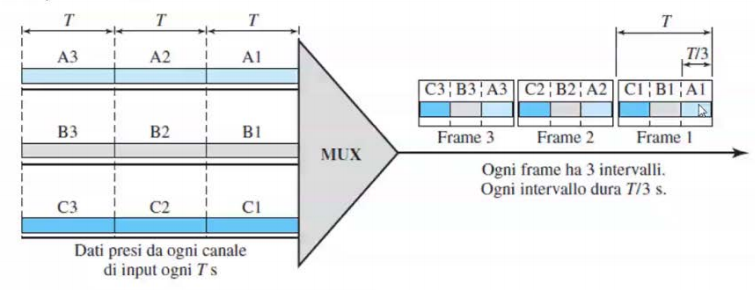
\includegraphics[scale=0.6]{images/TDM_Sincrono.png}
                        \end{center}
                    
                        In particolare, il TDM sincrono può essere \textit{multilivello} (utilizzato quando la velocità delle linee di input sono l'una multiplo dell'altra) e \textit{multiturno} (Alloca più di un turno ad un canale che è più veloce degli altri. Le velocità devono essere tutte multiple di un'unità di base).
                        
                        \vspace{3mm}
                        
                        Il vantaggio del TDM sincrono è la facilità di individuazione dei singoli canali; lo svantaggio è lo spreco di intervalli.
                    
                    \item
                        Nel \textbf{TDM statistico}, \textbf{gli intervalli sono assegnati dinamicamente}. Se un canale non ha dati, l'intervallo viene usato da un altro canale.
                        
                        \vspace{3mm}
                        
                        Il vantaggio del TDM statistico è che usa sempre gli intervalli. Lo svantaggio è che è difficile individuare i singoli canali logici.
                \end{itemize}
        \end{itemize}

        L'implementazione del multiplexing TDM è più complesso di quello FDM. \textbf{La sincronizzazione fra multiplexer e demultiplexer è un problema fondamentale.} Se non sono sincronizzati, l'appartenenza dei bit ai canali logici verrà falsata. 
        
        La soluzione è inserire uno o più \textbf{bit di sincronizzazione} nei frame (anche solo uno, il cui valore si alterna fra 0 e 1).
\section{Commutazione}
    Come ormai sappiamo bene, una rete è un insieme di dispositivi connessi tra di loro in base alla topologia adottata (nella mesh, canale punto-punt per ogni coppia di dispositivi; in alternativa, nella topologia a stella, vi è un nodo centrale e un canale fra tale nodo e ogni altro dispositivo). 
    
    La connessione è tale da connettere \textit{ogni} coppia di dispositivi. Nella realtà, quest'idea non è praticabile. Il numero e la lunghezza dei collegamenti costituirebbero costi troppi elevati. La soluzione è lo \textbf{switching}, cioè la commutazione.
    
    \vspace{3mm}
    
    Per connettere un insieme di nodi terminali (\textit{stazioni}), vengono utilizzati dei \textbf{nodi speciali interconnessi} (\textit{switch}), cioè dei dispositivi capaci di \textbf{creare connessioni temporanee} fra due o più stazioni connesse agli switch. Il loro utilizzo è limitato alla creazione di connessioni temporanee. Uno switch ha varie modalità di funzionamento, dette \textbf{commutazioni}.
    
    \subsection{Categorie di commutazioni}
    
        Le \textit{categorie di commutazioni} sono:
        
        \begin{itemize}
            \item 
                Reti a commutazione
            
            \begin{itemize}
                \item 
                    Reti a commutazione di circuito
                    
                \item 
                    Reti a commutazione di messaggio
    
                \item 
                    Reti a commutazione di pacchetto
                
                    \begin{itemize}
                        \item 
                            Reti a datagram
                            
                        \item 
                            Reti a circuito virtuale
                    \end{itemize}
            \end{itemize}
        \end{itemize}
    
        \subsubsection{Reti a commutazione di circuito}
                    
            La commutazione avviene nello \textbf{strato fisico}.
                
            Prima di iniziare la comunicazione, le stazioni devono effettuare una prenotazione delle risorse necessarie per la comunicazione. \textbf{Gli switch prenotano le risorse e definiscono il percorso}; tali risorse devono rimanere dedicate a questa connessione per tutta la durata del trasferimento dei dati, fino alla fase di eliminazione del circuito.
                
            \vspace{3mm}    
            
            I dati trasferiti tra due stazioni non sono divisi in pacchetti, ma spediti in un flusso continuo dalla stazione mittente a quella destinataria.
                
            Inoltre, non c'è bisogno di indirizzamento durante il trasferimento dei dati. Gli switch instradano i dati in base al canale riservato nella fase di instaurazione del circuito

            \vspace{3mm}
            
            I problemi principali delle reti a commutazione di circuito sono la scarsa efficienza dovuta al ritardo di rete, all'assenza di tempo di attesa negli switch e ad un generaler ritardo dovuto al tempo necessario ad instaurare il circuito, trasferire i dati ed eliminare il circuito. Il ritardo coincide con la somma fra tempo di propagazione della richiesta della stazione sorgente, il tempo necessario a trasferire la richiesta, il tempo di propagazione della risposta della stazione destinataria e il tempo per trasferire la risposta.

            \vspace{3mm}

            \textbf{Esempio tipico di commutazione di circuito}
                
            \begin{center}
                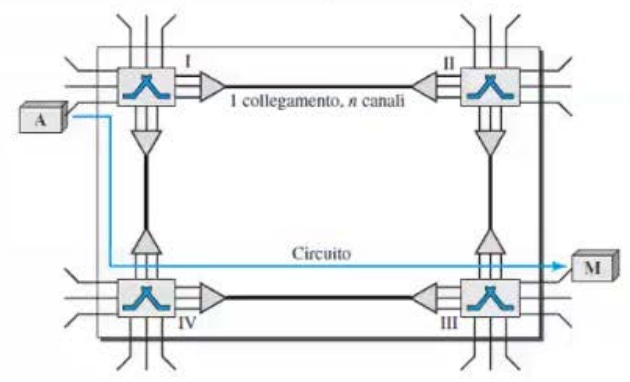
\includegraphics[scale=0.75]{images/Circuito_Fase1.png}
            \end{center}
                
            \textbf{Fase I - Instaurazione della connessione}
                
            \vspace{3mm}
                
            \textit{Fase I.A - Obiettivo:} $A$ spedisce una richiesta all'indirizzo $M$.
                
            \begin{itemize}
            
                \item
                    $A$ spedisce la richiesta allo switch $I$ con l'indirizzo di $M$.
                    
                \item
                    $I$ spedisce la richiesta allo switch $IV$.
                    
                \item
                    $IV$ spedisce la richiesta allo switch $III$.
                    
                \item
                    $III$ spedisce la richiesta ad $M$.
                    
            \end{itemize}
            
            \textit{Fase I.B - Obiettivo:} $M$ accetta la richiesta
            
            \vspace{3mm}
            
            $M$ risponde a $III$, che risponde a $IV$, che risponde a $I$, che risponde ad $A$.
            
            \vspace{3mm}
            
            \textbf{Fase II - Spedizione dei dati}
            
            \vspace{3mm}
            
            $A$ spedisce i dati indicando il circuito instaurato nella prima fase. Adesso, gli switch conoscono la posizione di $M$ e sanno che i dati devono arrivare lì, partendo da $A$, sfruttando il canale dedicati ai dati.
            
            \vspace{3mm}
            
            \textbf{Fase III - Chiusura della connessione}
            
            \vspace{3mm}
            
            \textit{ Fase III.A - Obiettivo:} $A$ chiude la connessione.
            
            \begin{itemize}
                \item 
                    $A$ spedisce la richiesta di chiusura allo switch $I$
                
                \item
                    $I$ libera le risorse riservate
                    
                \item
                    $I$ spedisce la richiesta di chiusura allo switch $IV$
                    
                \item
                    $IV$ libera le risorse riservate
                    
                \item
                    $IV$ spedisce la richiesta di chiusura allo switch $III$
                    
                \item
                    $III$ libera le risorse riservate
                    
                \item
                    $III$ spedisce la richiesta di chiusura a $M$
            \end{itemize}
            
        \subsubsection{Reti a datagram}
        
            I messaggi devono essere divisi in pacchetti, detti \textbf{datagram}, a lunghezza variabile o fissa.
            
            La grandezza dei pacchetti è determinata dalla rete e dal protocollo che ne gestisce il funzionamento. Non c'è allocazione di risorse per un pacchetto; non ci sono canali riservati, né risorse riservate negli switch. I pacchetti sono gestiti tramite FIFO.
            
            \vspace{3mm}
            
            I pacchetti vengono instradati verso la loro destinazione tramite le \textbf{tavole di routing}, che contiene informazioni di instradamento in funzione dell'indirizzo di destinazione.
            
            \vspace{3mm}
            
            I ritardi di una rete a datagram possono essere maggiori di quelli in una rete a circuito. Ogni pacchetto potrebbe subire un ritardo negli switch prima di essere inoltrato.
            
        \subsubsection{Reti a circuito virtuale}
        
            Sono una via di mezzo fra la commutazione di circuito e la commutazione di datagram e sintetizza le caratteristiche di entrambe.
            
            I dati sono divisi in pacchetti, ogni pacchetto contiene un indirizzo di destinazione. Le risorse necessarie possono essere allocate dinamicamente.
            
            \vspace{3mm}
            
            Analogamente alle reti a commutazione di circuito, inoltre, vi è una fase di instaurazione (in cui uno switch crea una riga nella tavola di routing per il circuito virtuale dela connessione richiesta) e di chiusura della connessione, oltre al trasferimento dei dati. 
            
            Tutti i pacchetti seguono lo stesso percorso, stabilito durante la connessione. Le risorse necessarie sono prenotate, come nella commutazione di circuito. E' implementata nello strato di collegamento, fisico e di rete.
            
            \vspace{3mm}
            
            Utilizza due tipi di instradamento: \textit{globale} (qualsiasi nodo della rete deve avere un indirizzo globale) e \textit{locale} (degli identificatori di circuito virtuali - VCI - vengono usati per trasferire dati; i VCI sono numeri con significati locali, in base alla coppia di switch: in pratica, combina switch a switch).
            
    \subsection{Struttura dello switch}
    
        La tecnologia attuale per gli switch di una rete a circuito virtuale utilizza \textbf{switch a divisione di spazio} (crossbar, switch a più livelli) e \textbf{switch a divisione di tempo}.
        
        \vspace{3mm}
        
        Negli switch a divisione di spazio, i circuiti sono separati fisicamente. Ogni switch occupa il proprio spazio, e originariamente furono progettati per reti analogiche. 
        
        Gli switch a crossbar dispongono $n$ linee di input verso $m$ linee di output. I punti di incrocio sono $n*n$. Gli switch a più livelli combinano vari switch crossbar a più livelli, appunto. Il vantaggio degli switch a divisione di spazio è la comunicazione istantanea; lo svantaggio è il numero di punti di incrocio necessari affinché lo switch non sia bloccante.
        
        Gli switch a divisione di tempo utilizzano il TDM con tecnologia a scambio di intervalli temporali (TSI). Il vantaggio degli switch a divisione di tempo è che non richiede punti di incrocio; lo svantaggio è che la gestione di ogni connessione crea ritardi.
        
        Infine, gli \textbf{switch misti} combinano gli switch a divisione di spazio e divisione di tempo.

\section{Domande frequenti all'esame}

\begin{itemize}
    \item
    Costruire una tavola di routing e descrivere l'algoritmo di routing basato sullo strato di collegamento o sul vettore delle distanze, mostrandone il funzionamento; descrivere inoltre il problema dell'instabilità (relativo a un ciclo di due nodi) e come può essere risolto
    
    \item
    Mostrare in modo dettagliato il processo di inoltro di un datagram
    
    \item
    Frammentare un datagram secondo certi dati forniti dalla traccia
    
    \item
    Descrivere caratteristiche e funzionalità del protocollo TCP
    
    \item
    Descrivere il controllo del flusso nel TCP
    
    \item
    Descrivere il protocollo ARP, il suo funzionamento e il formato dei messaggi scambiati
    
    \item
    Descrivere il protocollo ICMP, in particolare i messaggi di notifica degli errori
    
    \item
    Creare sottoblocchi di una possibile allocazione di un blocco di indirizi ad un gruppo di $n$ persone
    
    \item
    Mostrare i tre segmenti TCP utilizzati nella fase di apertura della connessione nelle ipotesi di certi valori \textit{rwnd}
    
    \item
    Descrivere i concetti fondamentali relativi alla velocità di trasferimento durante la trasmissione dati, i limiti e le differenze fra il Teorema di Nyquist e il Teorema di Shannon; inoltre, data la banda $B$ e l'$SNR$ di un canale, determinare a quale velocità si può spedire e quanti livelli del segnale si possono utilizzare. 
    
    \item
    Descrivere il multiplexing e le tecniche fondamentali per implementarlo
    
    \item
    Descrivere i protocolli per canali senza rumore dello strato di collegamento
    
    \item
    Descrivere il funzionamento del DNS
    
    \item
    Descrivere le tecniche di codifica unipolari e polari utilizzate nella codifica digtale-digitale
    
    \item
    Descrivere le reti di commutazione di circuito
    
    \item
    Descrivere i codici lineari utilizzati per la correzzione degli errori, evidenziando le principali differenza tra codici a parità, codici a parità bidimensionale e codici di Hamming
    
    \item
    Descrivere i protocolli RARP, BOOT e DHCP
    
    \item
    Descrivere il comando traceroute nei sistemi Unix mostrandone il funzionamento su una rete d'esempio
    
    \item
    Sottolineare le differenze fra segnali semplici e composti
    
    \item
    Dato un indirizzo IP, determinare il numero di indirizzi nella rete, nonché il primo e l'ultimo indirizzo del blocco
    
    \item
    Descrivere la procedura di handshake in una connessione TCP
    
    \item
    Descrivere i concetti fondamentali relativi alle codifiche analogico-digitale e digitale-analogico
    
    \item
    Descrivere le differenze sostanziali fra reti a commutazione di circuito e reti a commutazione di pacchetto
    
    \item
    Descrivere il formato di un datagram IP
    
    \item
    Descrivere le misure utilizzate per misurare l'efficienza di una rete
    
    \item
    Descrivere le funzionalità del protocollo IP, descrivendone in dettaglio la frammentazione; descrivere i campi dell'intestazione IPv4
    
    \item
    Si fornisca la notazione decimale e binaria di un certo indirizzo IPv4; trovare l'errore in un indirizzo IPv4
    
    \item
    Descrivere il meccanismo di congestione nel TCP
    
    \item
    Descrivere in dettaglio i campi dell'header di un segmento TCP e spiegare i meccanismi di instaurazione e chiusura delle connessioni TCP
    
    \item
    Descrivere il funzionamento del three-way handshake
    
    \item
    Descrivere il meccanismo di indirizzamento con e senza classi
    
    \item
    Descrivere i protocolli ALOHA e CSMA
    
    \item
    Descrivere il protocollo UDP
    
    \item
    Svolgere un esercizio pratico sulla congestione nel TCP (\textit{slow-start}, \textit{
ssthresh})
\end{itemize}

\end{document}
